\section{Implementation}
\subsection{Package structure}
Package structure decision was as important task in \textbf{\textit{PokèMongo}}, we wanted to ensure an high level of readability and maintainability.
Although the classical “root package” which specifies the “domain.company.projet”, in our case “it.unipi.dii.lsmsd.pokemongo”, all the packages are structured \textit{by layers}. In this way, we decided to name the packages according to they function architecturally rather than their identity according to the business domain. Here the structure: 

\begin{figure}[H]
	\centering
	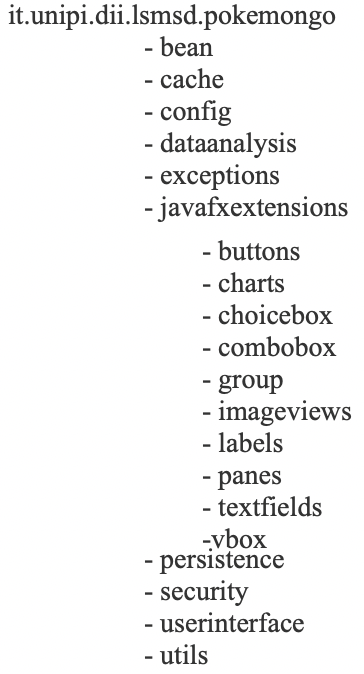
\includegraphics[width= 0.3\textwidth]{img/package_structure.png}
	\caption{Package Structure}
\end{figure}

We tried to maintain the name of the packages as simple as possible, and in a way they are all easy to read and to understand.
We also followed the convention of having the first character in the package names in lower case, in order to avoid conflicts with class or interface names.

\subsubsection{Package Analysis: Bean}
The \textit{bean} package contains few classes that are used as beans while the application runs.

\begin{figure}[H]
	\centering
	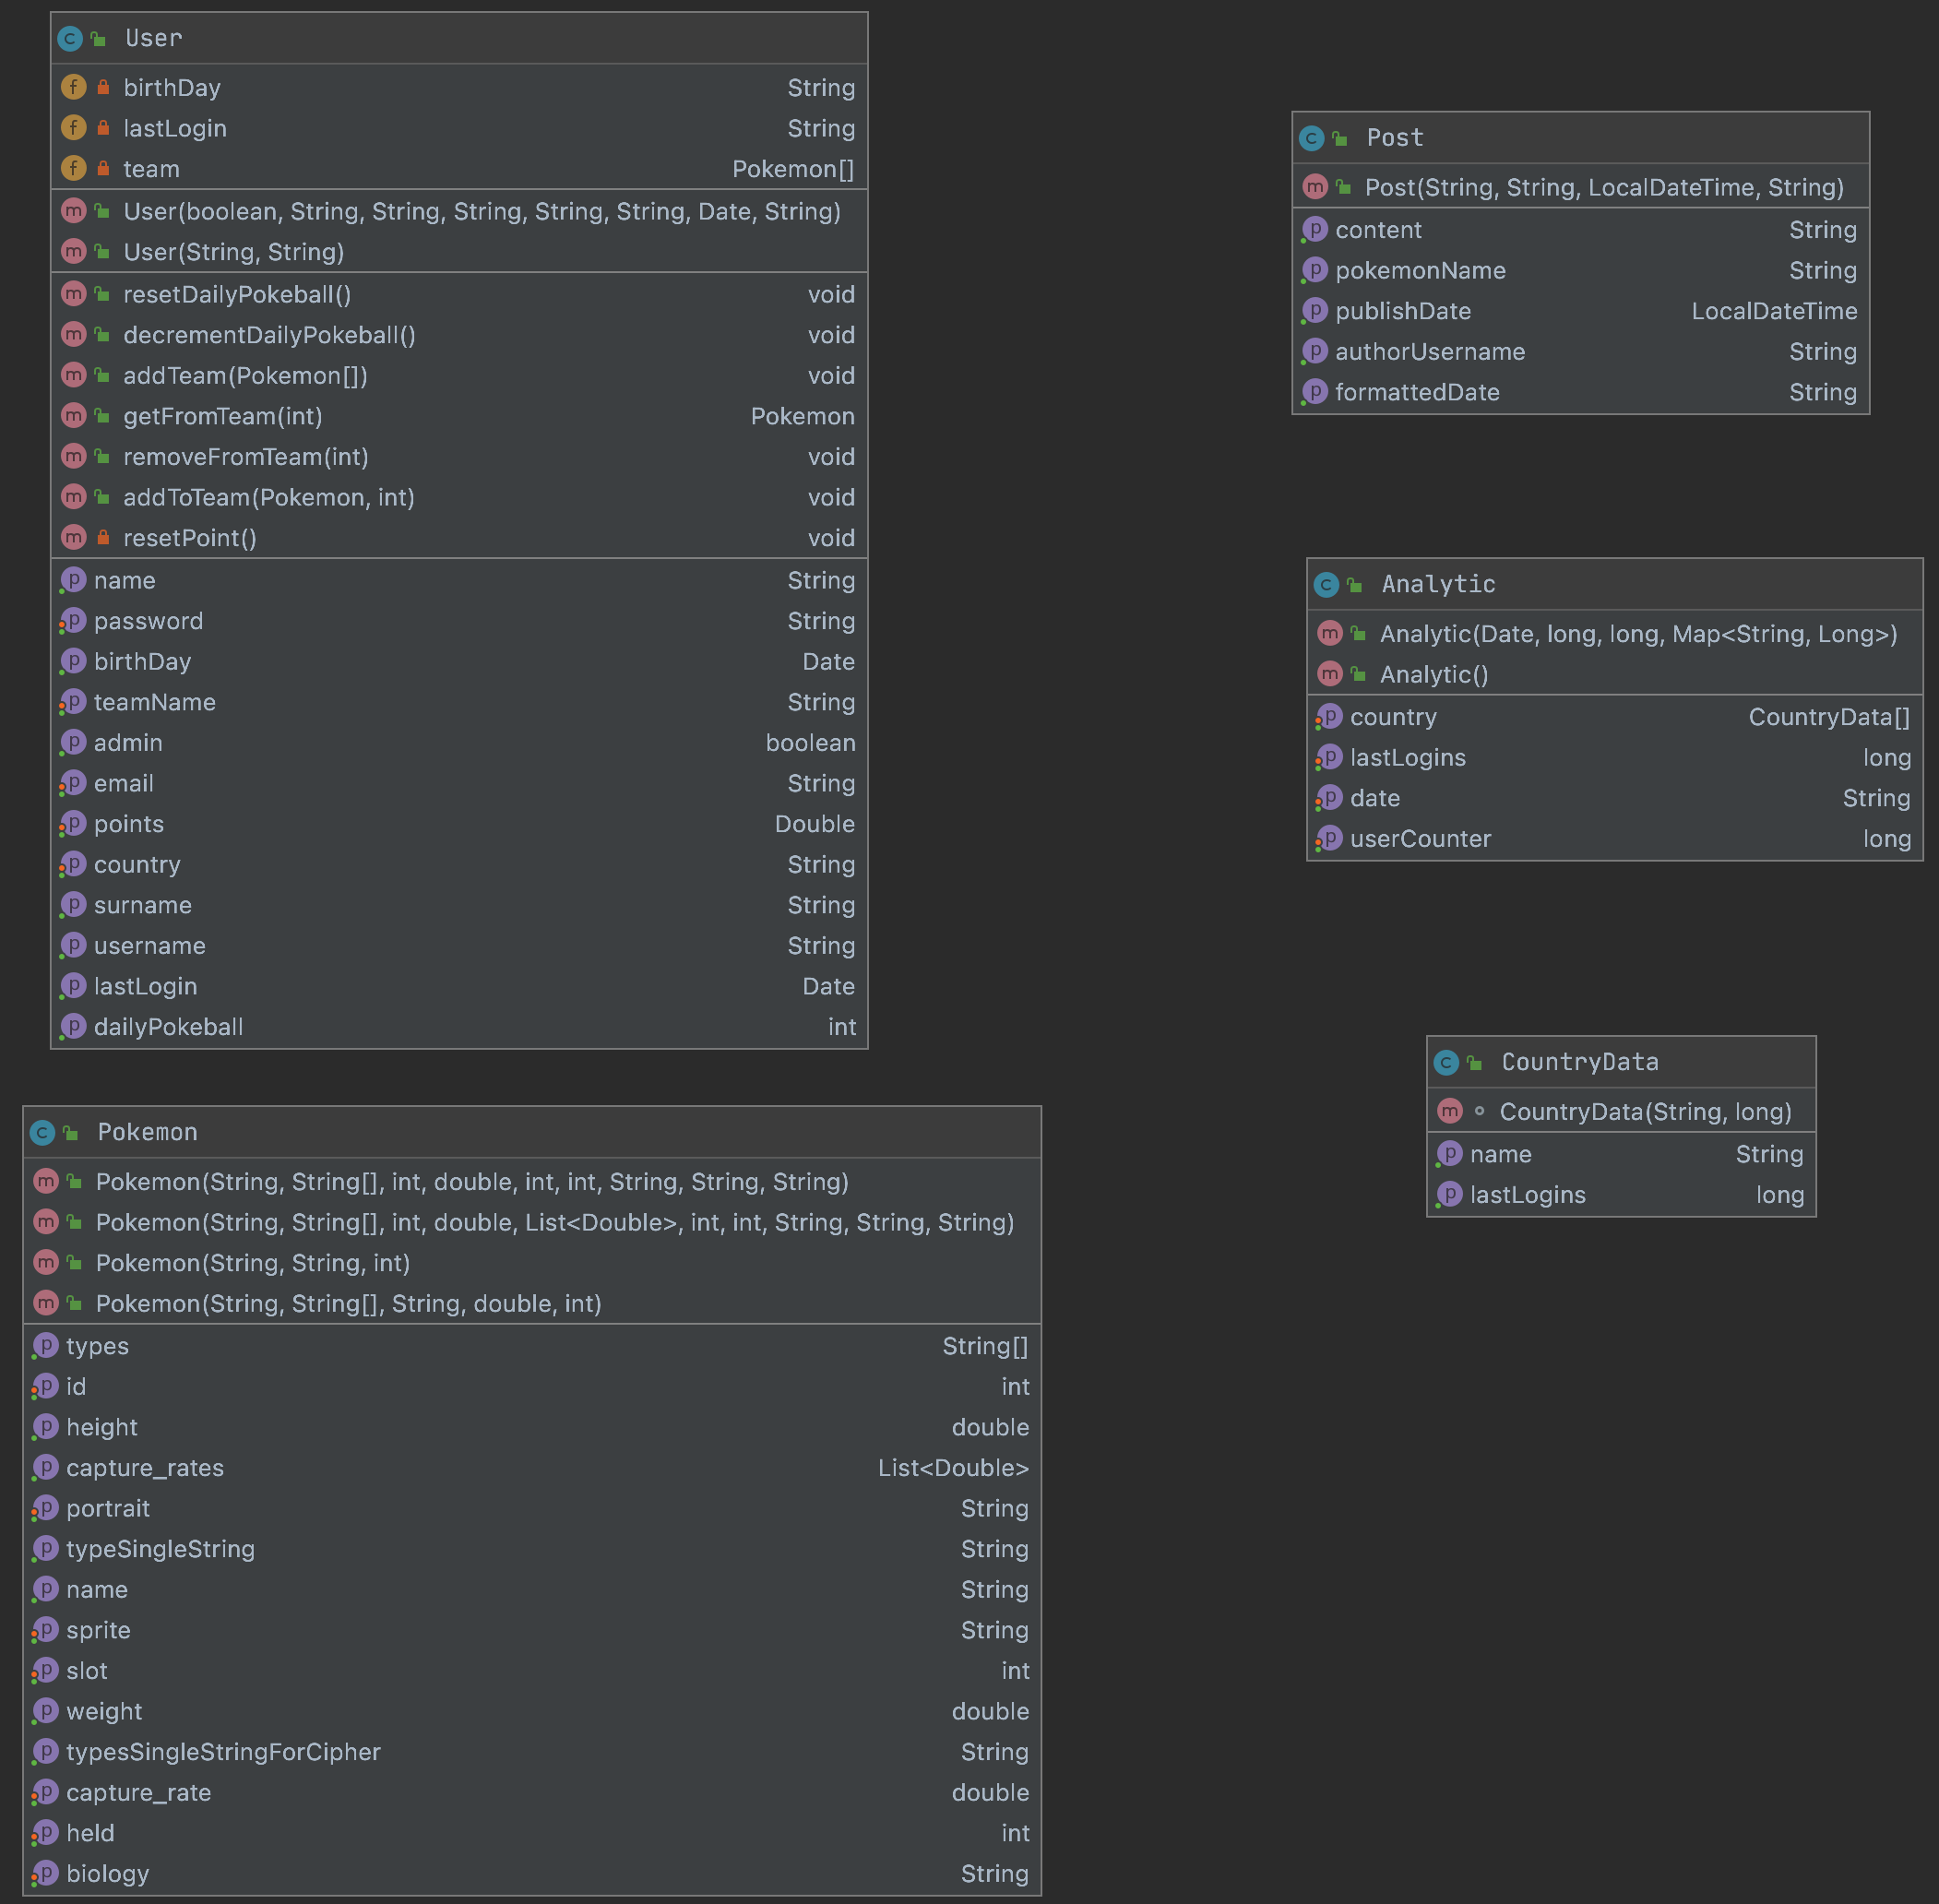
\includegraphics[width=0.9\textwidth]{img/bean_package.png}
	\caption{Bean Package Class Structure}
\end{figure}

\begingroup
\setlength{\tabcolsep}{10pt} % Default value: 6pt
\renewcommand{\arraystretch}{1.5} % Default
\begin{center}
	\begin{longtable}{| m{9em} | m{22em} |} 
		\hline
		\textbf{Class Name} & \textbf{Short Description} \\ [0.5ex] 
		\hline
		User & The \textbf{User} class is used for instantiating object that refers to a specific user\\ 
		\hline
		Pokemon & The \textbf{Pokemon} class is used for instantiating object that refers to a specific Pokemon\\
		\hline
		Post & The \textbf{Post} class is used for instantiating object that refers to a specific \textbf{Post}. Responses (aka sub-Posts) are considered post also.\\
		\hline
		Analytic & This class is used for containing the information regarding a particular day.\\
		\hline
		CountryData & Used in the \textbf{Analytic} bean, it contains the information regarding a single country and the analytic strictly associated to it.\\
		\hline
	\end{longtable}
\end{center}
\endgroup

\subsubsection{Package Analysis: Cache}
The \textit{cache} package contains classes that are helpful for caching images, we will talk about that in chapter 4.3.2. Despite what written above, this is one of the few packages that has a feature logic structure inside. We maintain in this package not only the classes/interface that handle the caching functionality, but also a javafx class extension which is \textit{PokemonImage}. This class is strictly connected to the caching systems, because it contains the image we want to cache. We decided to use this approach to have a cleaner look and an easier maintainability for the caching systems. 
\begin{figure}[H]
	\centering
	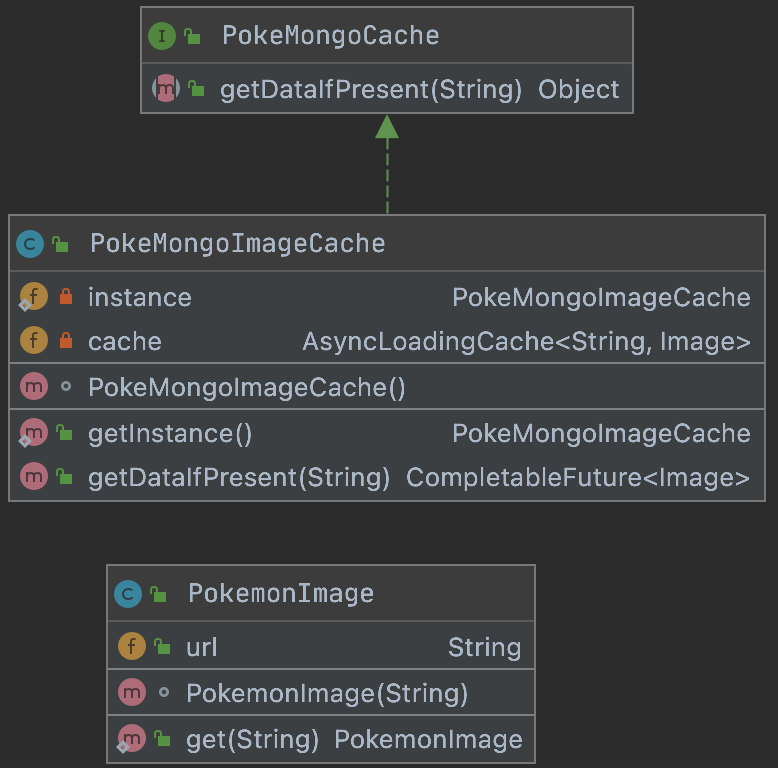
\includegraphics[width=0.4\textwidth]{img/cache_package.png}
	\caption{Cache Package Class Structure}
\end{figure}

\begingroup
\setlength{\tabcolsep}{10pt} % Default value: 6pt
\renewcommand{\arraystretch}{1.5} % Default
\begin{center}
	\begin{longtable}{| m{14em} | m{19em} |} 
		\hline
		\textbf{Class Name} & \textbf{Short Description} \\ [0.5ex] 
		\hline
		PokeMongoCache & Simply an interface.\\ 
		\hline
		PokeMongoImageCache & The implementation of the interface described.\\ 
		\hline
		PokemonImage & An Image (javaFX) extension that will contains the image we want to show to the user in the GUI.\\ 
		\hline
	\end{longtable}
\end{center}
\endgroup

\subsubsection{Package Analysis: dataAnalysis}
This package is used for instantiating factory structures about the data analysis we made in the project. Every factory is dependent of an interface. 

\begin{figure}[H]
	\centering
	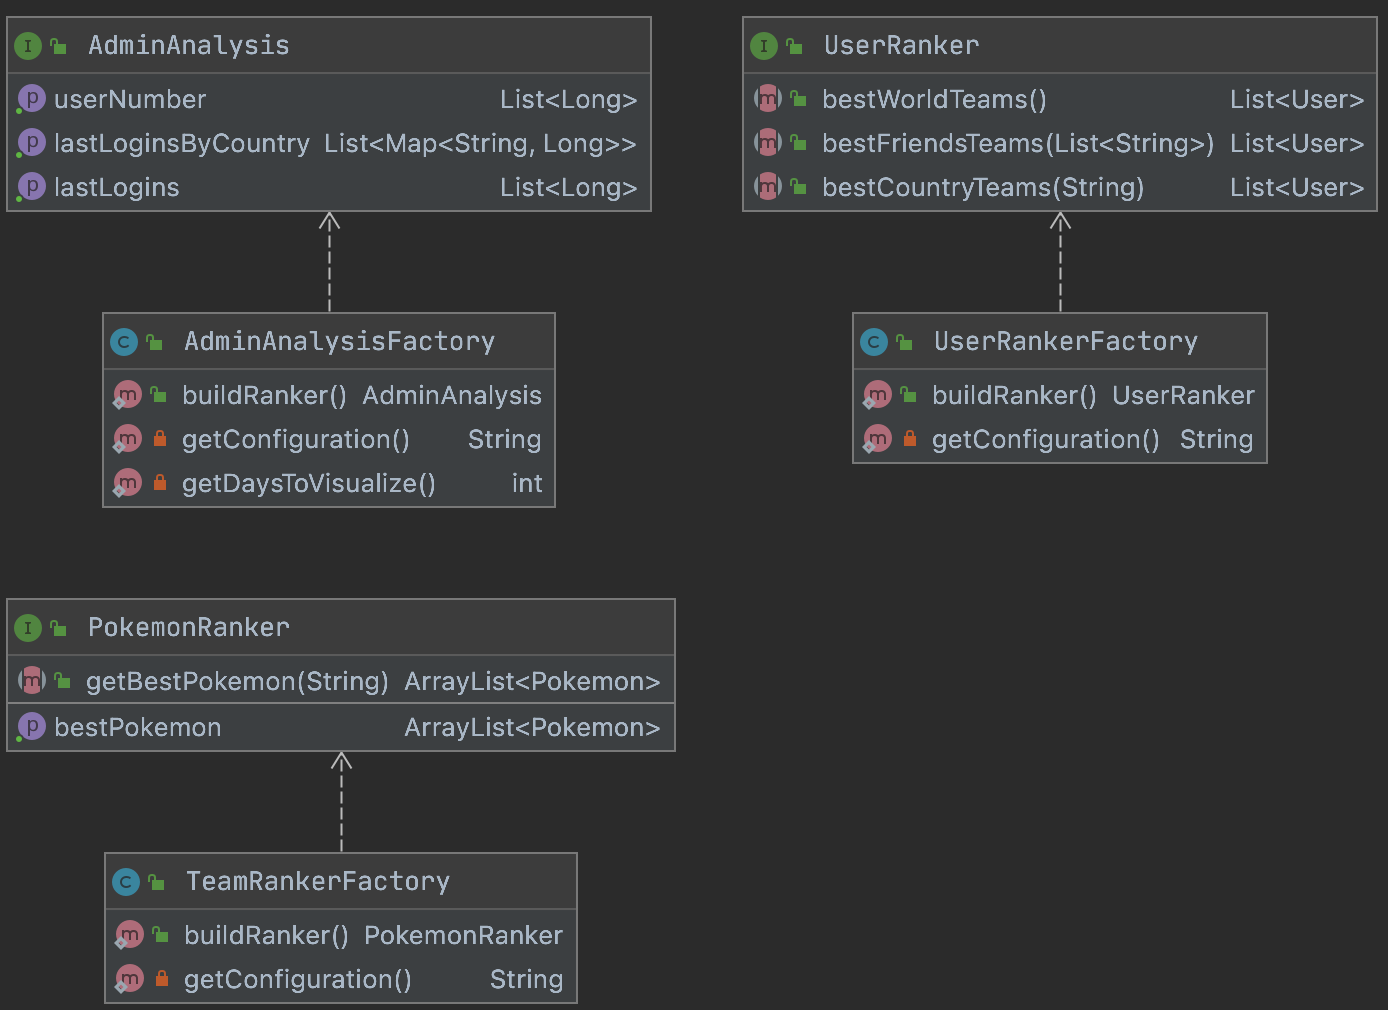
\includegraphics[width=0.7\textwidth]{img/dataAnalysis_package.png}
	\caption{dataAnalysis Package Class Structure}
\end{figure}

\begingroup
\setlength{\tabcolsep}{10pt} % Default value: 6pt
\renewcommand{\arraystretch}{1.5} % Default
\begin{center}
	\begin{longtable}{| m{14em} | m{19em} |} 
		\hline
		\textbf{Class Name} & \textbf{Short Description} \\ [0.5ex] 
		\hline
		AdminAnalytics &Simply an interface for the analytics related to the admin \textbf{User}\\ 
		\hline
		AdminAnalysisFactory & Has a static method that returns a specific implementation of the interface AdminAnalytics\\ 
		\hline
		UserRanker & Simply an interface for the analytics for \textbf{User} ranking.\\ 
		\hline
		UserRankerFactory & Has a static method that returns a specific implementation of the interface UserRanker\\ 
		\hline
		PokemonRanker & Simply an interface for the analytics for \textbf{Pokèmon} ranking\\ 
		\hline
		PokemonRankerFactory & Has a static method that returns a specific implementation of the interface PokemonRanker\\
		\hline
	\end{longtable}
\end{center}
\endgroup

\subsubsection{Package Analysis: exceptions}
This package contains classes that extend the class \textit{Exception} of Java. 
\begin{figure}[H]
	\centering
	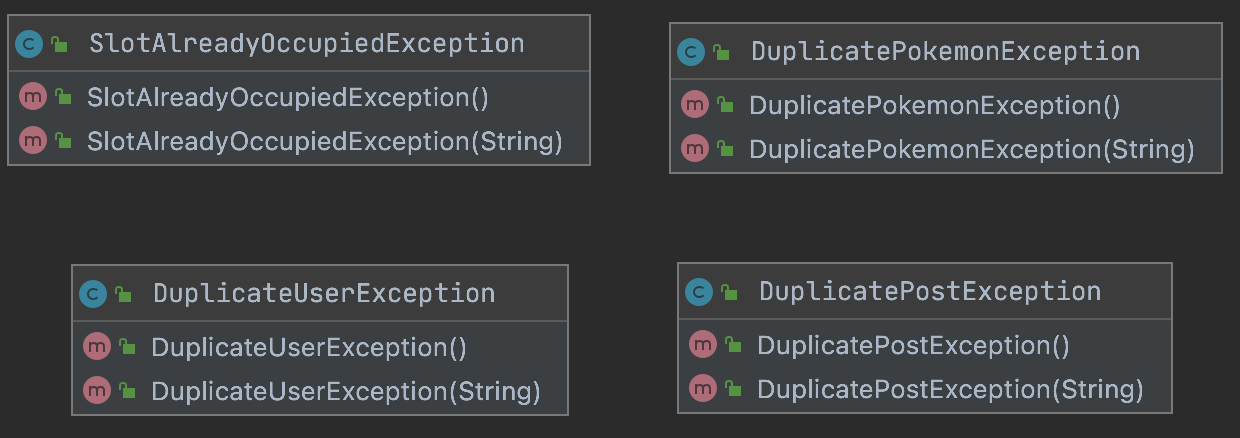
\includegraphics[width=0.7\textwidth]{img/exceptions_package.png}
	\caption{Exceptions Package Class Structure}
\end{figure}

\begingroup
\setlength{\tabcolsep}{10pt} % Default value: 6pt
\renewcommand{\arraystretch}{1.5} % Default
\begin{center}
	\begin{longtable}{| m{14em} | m{19em} |} 
		\hline
		\textbf{Class Name} & \textbf{Short Description} \\ [0.5ex] 
		\hline
		SlotAlreadyOccupiedException & Exception thrown when a user try to catch a \textbf{Pokèmon} and he has the \textit{slot} he want to use already occupied by one other \textbf{Pokèmon}\\ 
		\hline
		DuplicatePokemonException & Exception thrown when an admin try to insert a \textbf{Pokèmon} that is already present\\ 
		\hline
		DuplicateUserException & Exception thrown when an anonymous \textbf{User} try to create a register \textbf{User}, but the \textit{username} he writes is already taken.\\ 
		\hline
		DuplicatePostException & Exception thrown if an identical \textbf{Post} is created\\ 
		\hline
	\end{longtable}
\end{center}
\endgroup

\subsubsection{Package Analysis: javafxextensions}
In this package are present 11 sub-packages, any of them related to a specific extension of a JavaFX Node.
\subparagraph{javafxextensions: buttons}
Here are present all the classes that extend \textit{Button} from JavaFX
\begin{figure}[H]
	\centering
	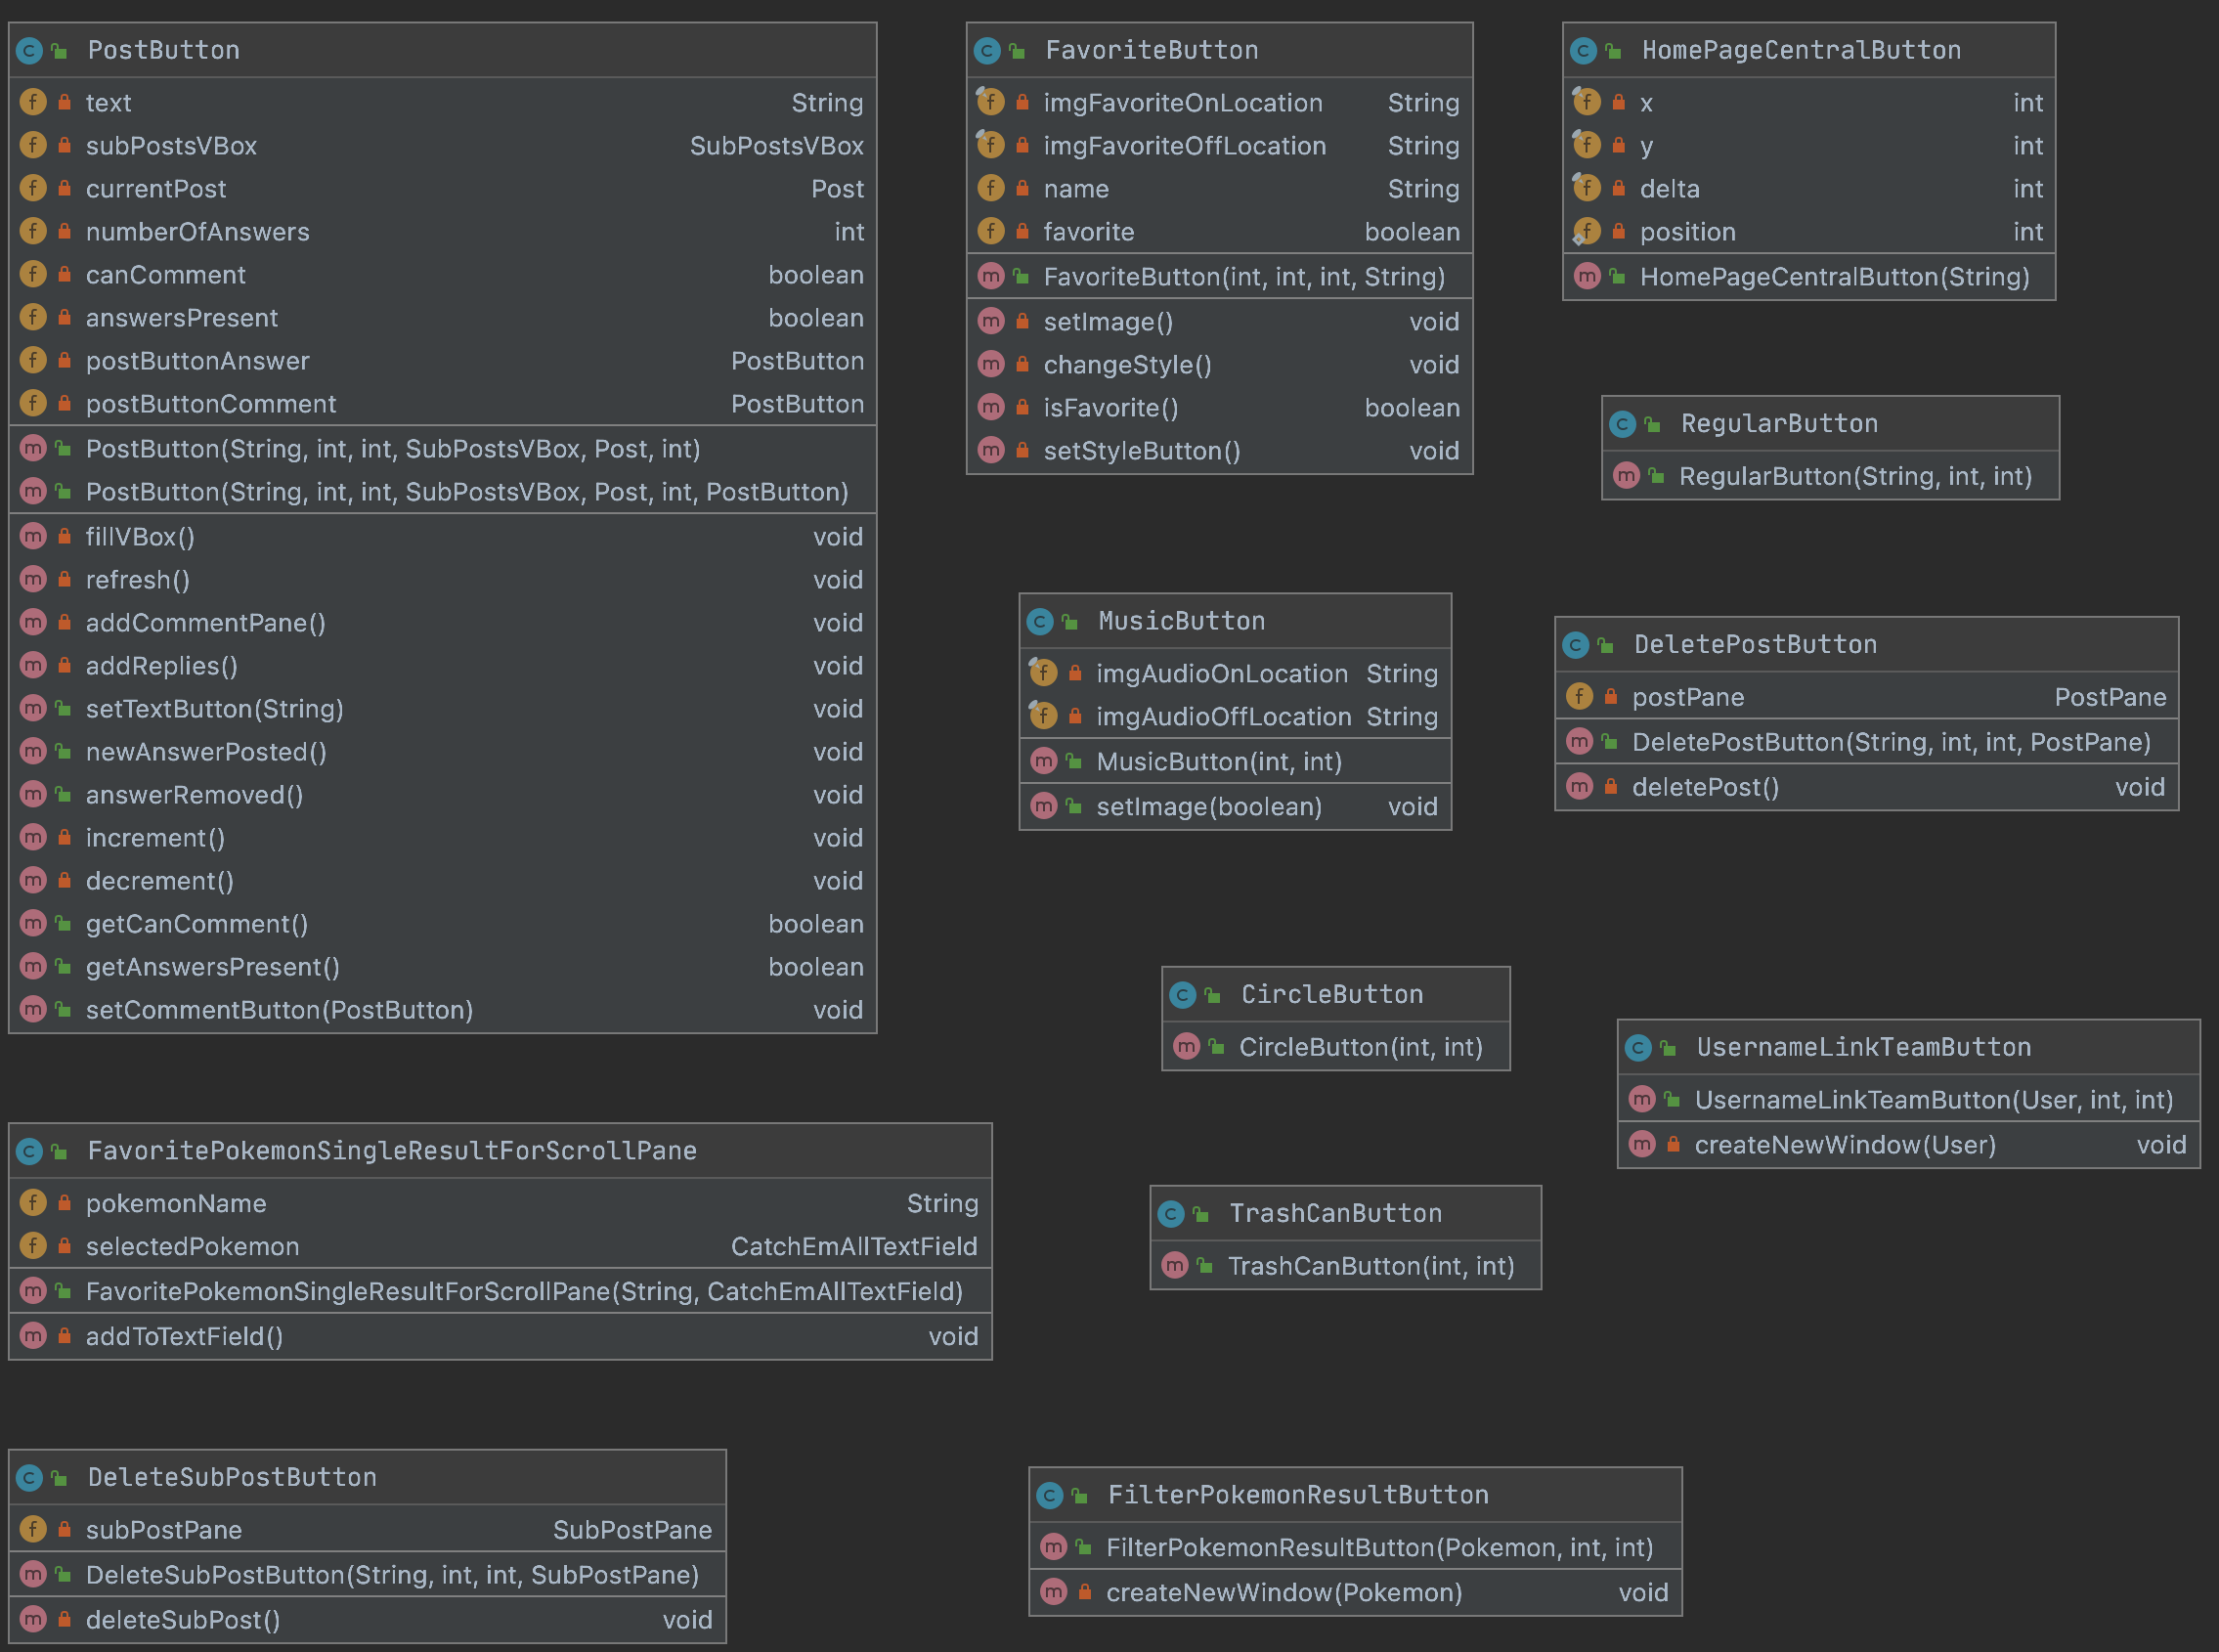
\includegraphics[width=0.7\textwidth]{img/javafx_buttons_package.png}
	\caption{javafxExtension/buttons Package Class Structure}
\end{figure}
\begingroup
\setlength{\tabcolsep}{10pt} % Default value: 6pt
\renewcommand{\arraystretch}{1.5} % Default
\begin{center}
	\begin{longtable}{| m{14em} | m{19em} |} 
		\hline
		\textbf{Class Name} & \textbf{Short Description} \\ [0.5ex] 
		\hline
		HomePageCentralButton & Specific button for the HomePage.\\ 
		\hline
		MusicButton & Button for turning the music on/off\\ 
		\hline
		RegularButton & For creating buttons like “BACK”, “SUBMIT”, etc…\\ 
		\hline
		TrashButton & Button for eliminating a \textbf{Pokèmon} in the \textbf{Team}\\ 
		\hline
		CircleButton & Helpful for creating button with a circular shape\\ 
		\hline
		PostButton & Specific button for submitting a comment in the post section of a \textbf{Pokèmon}\\
		\hline
		DeletePostButton & Button for deleting a \textbf{SubPost} (aka response)\\
		\hline
		FilterPokemonResultButton & Specific button for displaying the name of a \textbf{Pokèmon} in a query result. At the click it creates a new Stage with the information about the \textbf{Pokèmon} (check PokemonWindowGroup).\\
		\hline
		FavoritePokemonSingleResultFor ScrollPane & This button is used for showing the name of the \textbf{Pokèmon} than are Favourite. Clicking on it will be a shortcut for capturing the \textbf{Pokèmon} the button says about.\\
		\hline
		UsernameLinkTeamButton & Specific button for displaying the \textit{username} of a \textbf{User} in a query result. At the click it creates a new Stage with the team of the User (check TeamUserWindowGroup).\\
		\hline
	\end{longtable}
\end{center}
\endgroup

\subparagraph{javafxextensions: charts}
It contains a class that extends \textit{LineChart} from JavaFX.
\begin{figure}[H]
	\centering
	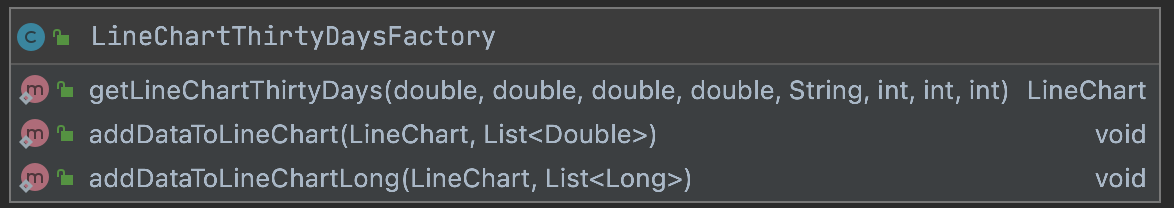
\includegraphics[width=0.7\textwidth]{img/javafx_charts_package.png}
	\caption{javafxExtensions/charts Package Class Structure}
\end{figure}
\begingroup
\setlength{\tabcolsep}{10pt} % Default value: 6pt
\renewcommand{\arraystretch}{1.5} % Default
\begin{center}
	\begin{longtable}{| m{14em} | m{19em} |} 
		\hline
		\textbf{Class Name} & \textbf{Short Description} \\ [0.5ex] 
		\hline
		LineChartThirtyDaysFactory & The class helps for the creation of different Line Charts, which can have different meanings (e.g. number of logins, number of users, …)  This is used for every plot in the application\\ 
		\hline
	\end{longtable}
\end{center}
\endgroup

\subparagraph{javafxextensions: choicebox}
It contains a class that extends LineChart from JavaFX.
\begin{figure}[H]
	\centering
	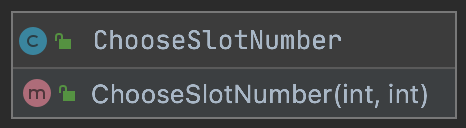
\includegraphics[width=0.5\textwidth]{img/javafx_choicebox_package.png}
	\caption{javafxExtensions/choicebox Package Class Structure}
\end{figure}

\begingroup
\setlength{\tabcolsep}{10pt} % Default value: 6pt
\renewcommand{\arraystretch}{1.5} % Default
\begin{center}
	\begin{longtable}{| m{14em} | m{19em} |} 
		\hline
		\textbf{Class Name} & \textbf{Short Description} \\ [0.5ex] 
		\hline
		ChooseSlotNumber & Choice box that lets the user to select the slot for saving the \textbf{Pokèmon} in captured\\ 
		\hline
	\end{longtable}
\end{center}
\endgroup

\subparagraph{javafxextensions: combobox}
A ComboBox can be seen as a ChoiceBox, the user select the elements in it in the same way.
\begin{figure}[H]
	\centering
	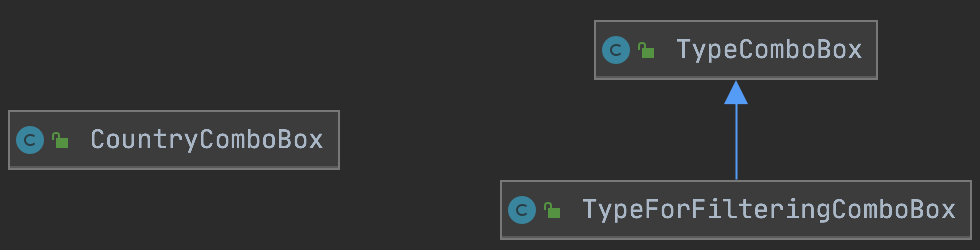
\includegraphics[width=0.8\textwidth]{img/javafx_combobox_package.png}
	\caption{javafxExtensions/combobox Package Class Structure}
\end{figure}
\begingroup
\setlength{\tabcolsep}{10pt} % Default value: 6pt
\renewcommand{\arraystretch}{1.5} % Default
\begin{center}
	\begin{longtable}{| m{14em} | m{19em} |} 
		\hline
		\textbf{Class Name} & \textbf{Short Description} \\ [0.5ex] 
		\hline
		CountryComboBox & Let the user to select the \textit{country}\\ 
		\hline
		TypeComboBox & General ComboBox for choosing the type of a \textbf{Pokèmon}\\ 
		\hline
		TypeForFilteringComboBox & Specific TypeComboBox for the filtering Pane.\\ 
		\hline
	\end{longtable}
\end{center}
\endgroup

\subparagraph{javafxextensions: group}
The group extensions are used for creating new windows with particular information regarding something. 
\begin{figure}[H]
	\centering
	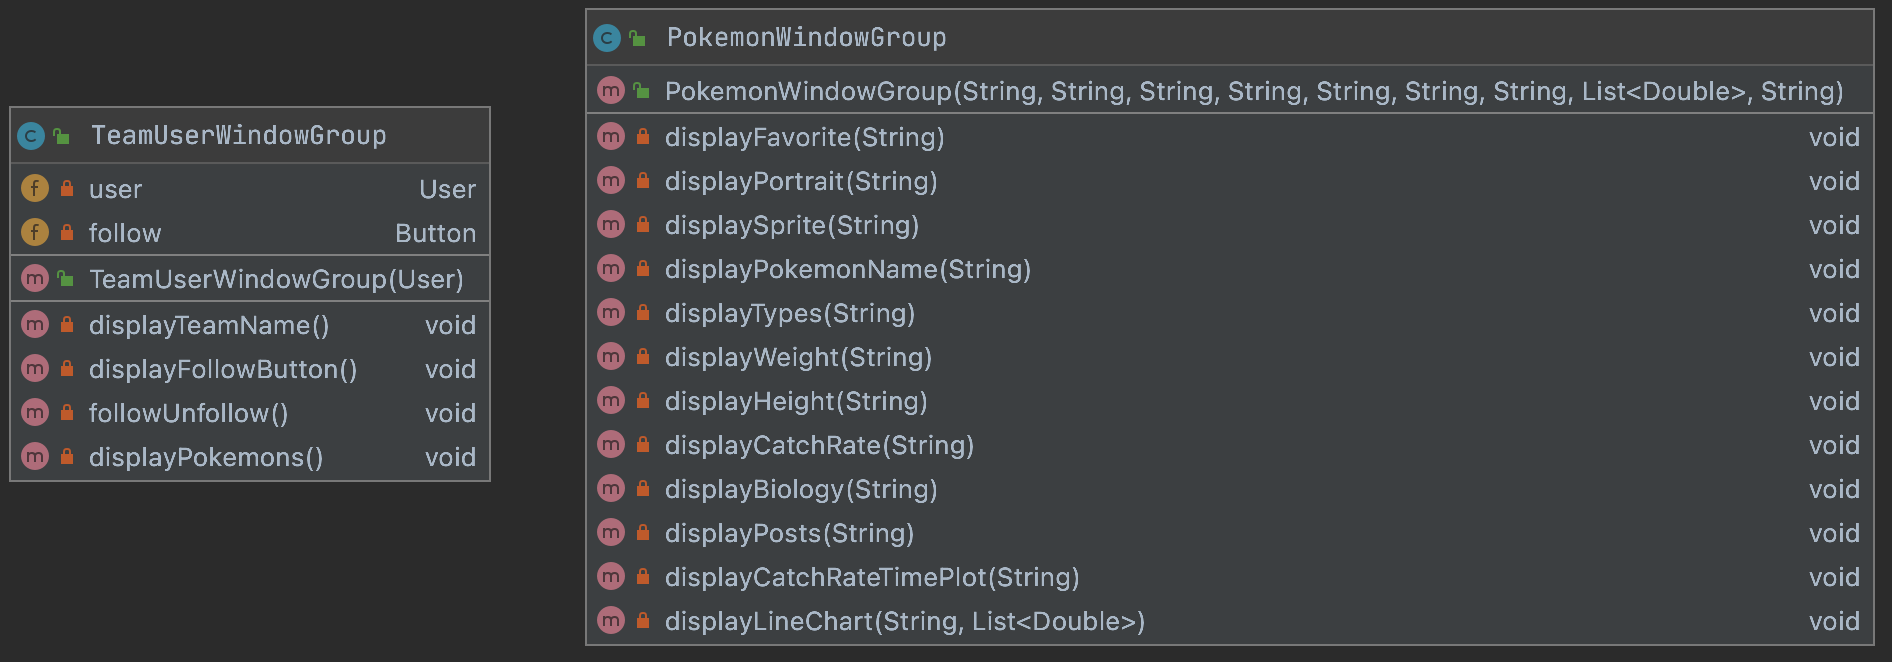
\includegraphics[width=0.8\textwidth]{img/javafx_group_package.png}
	\caption{javafxExtensions/group Package Class Structure}
\end{figure}
\begingroup
\setlength{\tabcolsep}{10pt} % Default value: 6pt
\renewcommand{\arraystretch}{1.5} % Default
\begin{center}
	\begin{longtable}{| m{14em} | m{19em} |} 
		\hline
		\textbf{Class Name} & \textbf{Short Description} \\ [0.5ex] 
		\hline
		TeamUserWindowGroup & Instantiates all the Node that are needed for creating the window which display the \textbf{Team} of a specific \textbf{User}\\ 
		\hline
		PokemonWindowGroup & Instantiates all the Node that are needed for creating the window which display the information of a specific \textbf{Pokèmon} along with the \textbf{Posts} related to it\\ 
		\hline
	\end{longtable}
\end{center}
\endgroup

\subparagraph{javafxextensions: imageviews}
Extensions of ImageView
\begin{figure}[H]
	\centering
	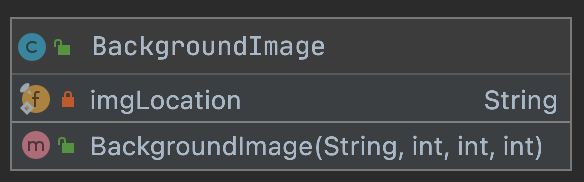
\includegraphics[width=0.5\textwidth]{img/javafx_imageviews_package.png}
	\caption{javafxExtensions/imageviews Package Class Structure}
\end{figure}
\begingroup
\setlength{\tabcolsep}{10pt} % Default value: 6pt
\renewcommand{\arraystretch}{1.5} % Default
\begin{center}
	\begin{tabular}{| m{14em} | m{19em} |} 
		\hline
		\textbf{Class Name} & \textbf{Short Description} \\ [0.5ex] 
		\hline
		BackgroundImage & Helpful for adding image in the background.\\ 
		\hline
	\end{tabular}
\end{center}
\endgroup

\subparagraph{javafxextensions: labels}
This package contains different types of labels useful for different situations.
\begin{figure}[H]
	\centering
	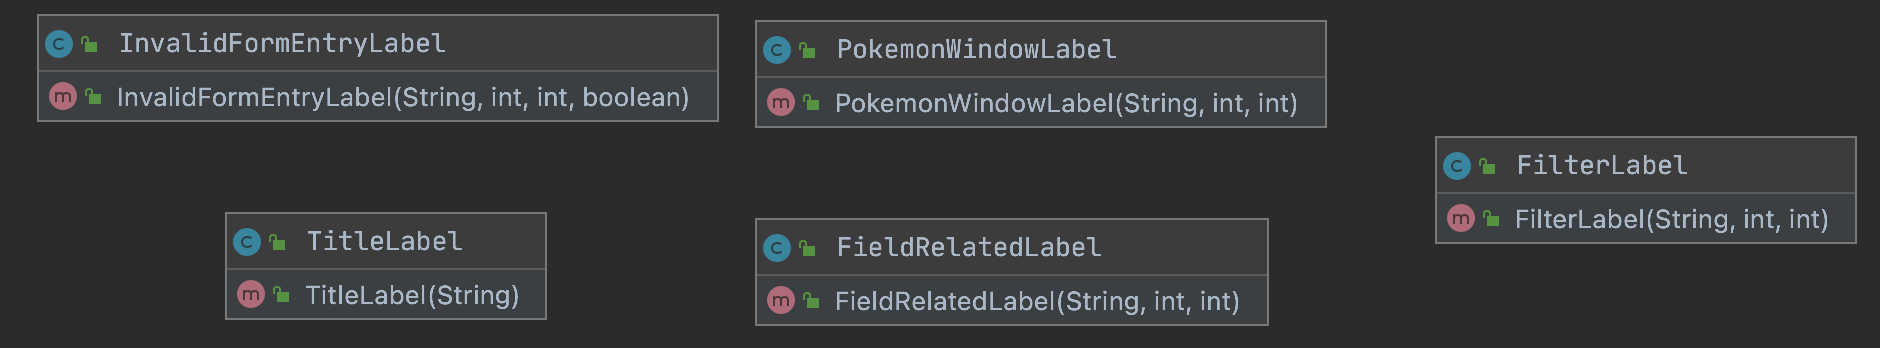
\includegraphics[width=0.8\textwidth]{img/javafx_labels_package.png}
	\caption{javafxExtensions/labels Package Class Structure}
\end{figure}
\begingroup
\setlength{\tabcolsep}{10pt} % Default value: 6pt
\renewcommand{\arraystretch}{1.5} % Default
\begin{center}
	\begin{tabular}{| m{14em} | m{19em} |} 
		\hline
		\textbf{Class Name} & \textbf{Short Description} \\ [0.5ex] 
		\hline
		InvalidFormEntryLabel & Used when an error occurs at the filling of an entry in a form.\\ 
		\hline
		PokemonWindowLabel & A specific Label that is used in the Stage created with the information of a specific \textbf{Pokèmon}\\ 
		\hline
		TitleLabel & Used for creating title in a prefix position.\\ 
		\hline
		FieldRelatedLabel & Used to indicate what a TextField is related to\\ 
		\hline
		FieldLabel & Used for the labels in the filter Pane\\ 
		\hline
	\end{tabular}
\end{center}
\endgroup

\subparagraph{javafxextensions: panes}
The Panes are the most important JavaFX extension we made in the project. The Panes help the system to be more modular. Modularity by the Panes is archived by dividing every complex components of the GUI in sub components that can be used and modified as stand alone (this gives us also an high level of maintainability). Only one type of Pane is standing separated by the others, inside the addPane package contained in the pane package, this because this pane is strictly connected to an enum that is present in that same folder (we just want to divide this particular enum, to the rest of the panes that, in fact, do not interact with it). 
\begin{figure}[H]
	\centering
	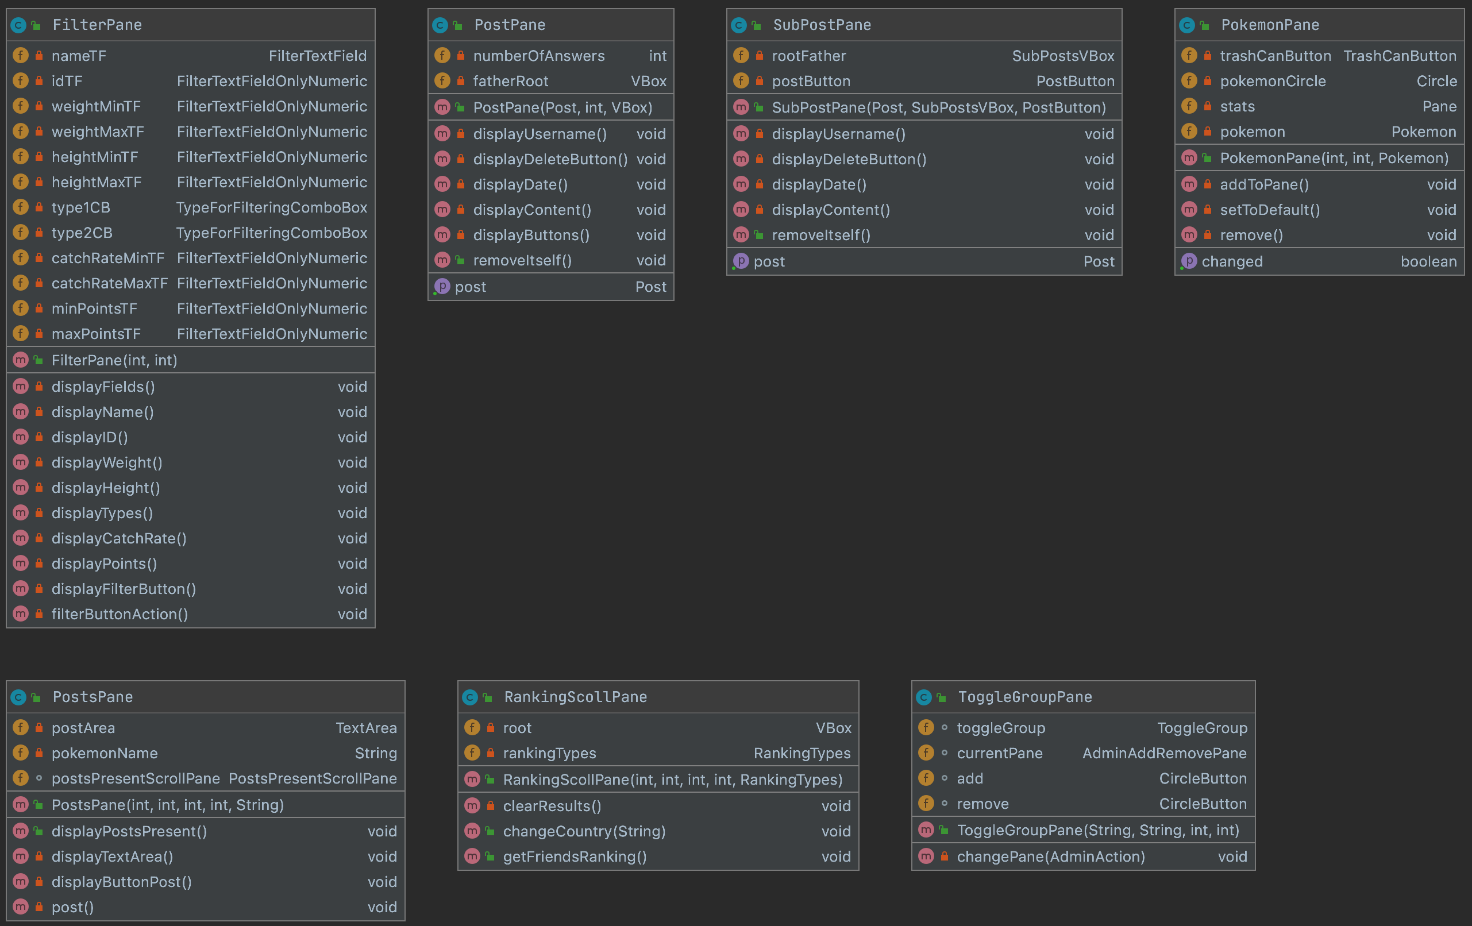
\includegraphics[width=\textwidth]{img/javafx_panes_package.png}
\end{figure}
\begin{figure}[H]
	\centering
	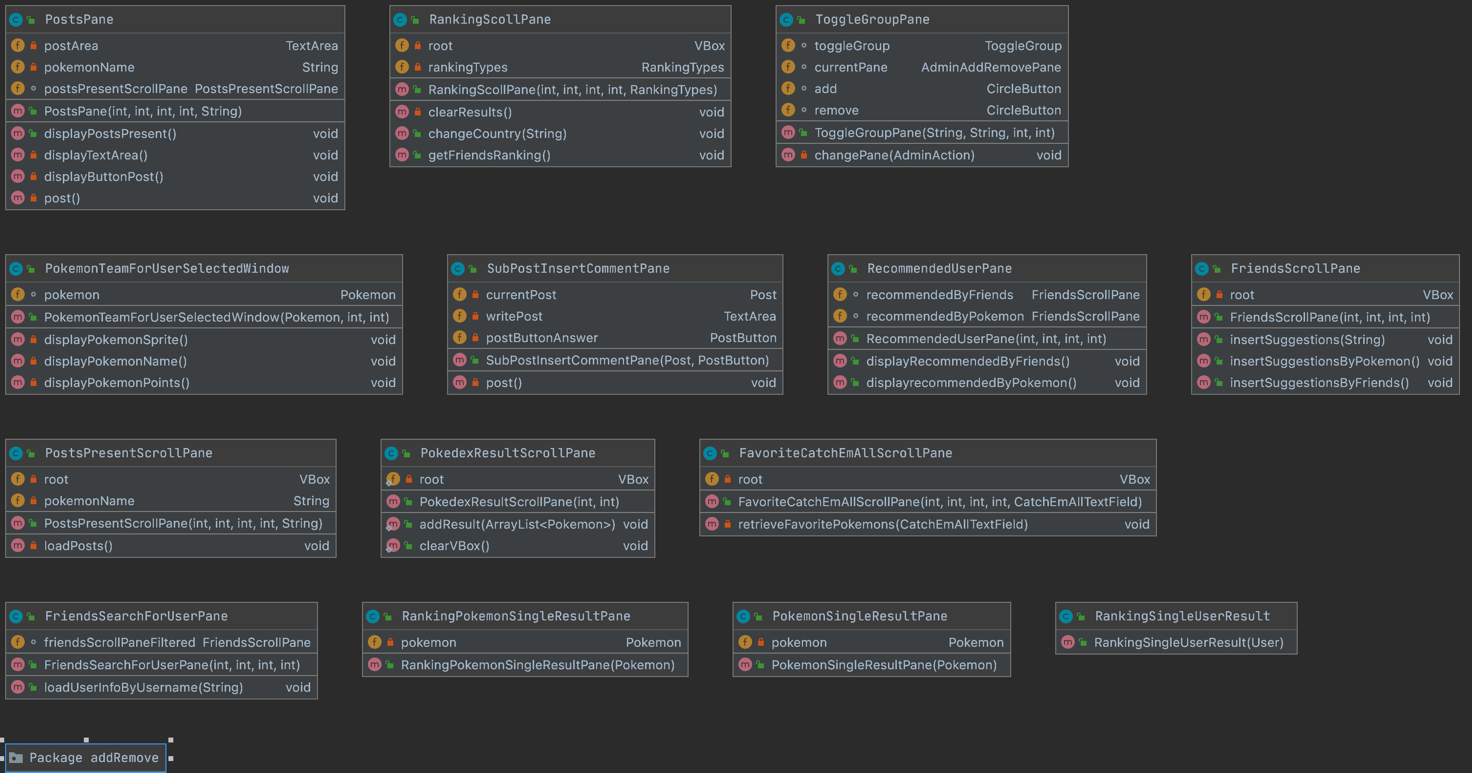
\includegraphics[width=\textwidth]{img/javafx_panes_package2.png}
	\caption{javafxExtensions/panes Package Class Structure}
\end{figure}
\begingroup
\setlength{\tabcolsep}{10pt} % Default value: 6pt
\renewcommand{\arraystretch}{1.5} % Default
\begin{center}
	\begin{longtable}{| m{14em} | m{19em} |} 
		\hline
		\textbf{Class Name} & \textbf{Short Description} \\ [0.5ex] 
		\hline
		RankingScrollPane & Pane that can be scrolled. It contains other panes that are specific for something (e.g. a \textbf{User}, a \textbf{Pokèmon}).\\ 
		\hline
		ToggleGroupPane & Specific pane for creating a toggle group\\ 
		\hline
		PokemonTeamForUserSelected Window & Specific pane for showing a single \textbf{Pokèmon} in the other \textbf{User} window.\\ 
		\hline
		SubPostInsertCommentPane & Specific pane that is used to create the Nodes for a response to a \textbf{Post}. The need of that comes by the fact the TextArea and the button in it should be horizontal to each other (impossible in the VBox this Pane it’s used).\\ 
		\hline
		RecommendedUserPane & Specific Pane for the recommended section in the Friends page.\\ 
		\hline
		FriendsScrollPane & Specific ScrollPane to visualize friends \textbf{Users} (an even the one recommended).\\ 
		\hline
		PostsPresentScrollPane & Specific ScrollPane to visualize a limited number of \textbf{Posts}.\\ 
		\hline
		PokedexResultScrollPane & Specific ScrollPane to visualize the result of a filtering operation.\\ 
		\hline
		FavoriteCatchEmAllScrollPane & Specific ScrollPane to visualize the \textbf{Pokèmon} set as favourite\\ 
		\hline
		FriendsSearchForUserPane & Specific pane for searching an user (Friends scene)\\ 
		\hline
		RankingPokemonSingleResult PaneSpecific & Specific pane to be inserted in a ScrollPane extension. It gives some information about the \textbf{Pokèmon} (used in the \textit{Ranking})\\ 
		\hline
		PokemonSingleResultPane & Specific pane to be inserted in a ScrollPane extension. It gives some information about the \textbf{Pokèmon} (used in the \textit{Pokedex})\\
		\hline
		RankingSingleUserResult & Specific pane to be inserted in a ScrollPane extension. It gives some information about the \textbf{Pokèmon} (used in the \textit{Ranking})\\
		\hline
	\end{longtable}
\end{center}
\endgroup

The addRemove package is characterized of these classes:
\begin{figure}[H]
	\centering
	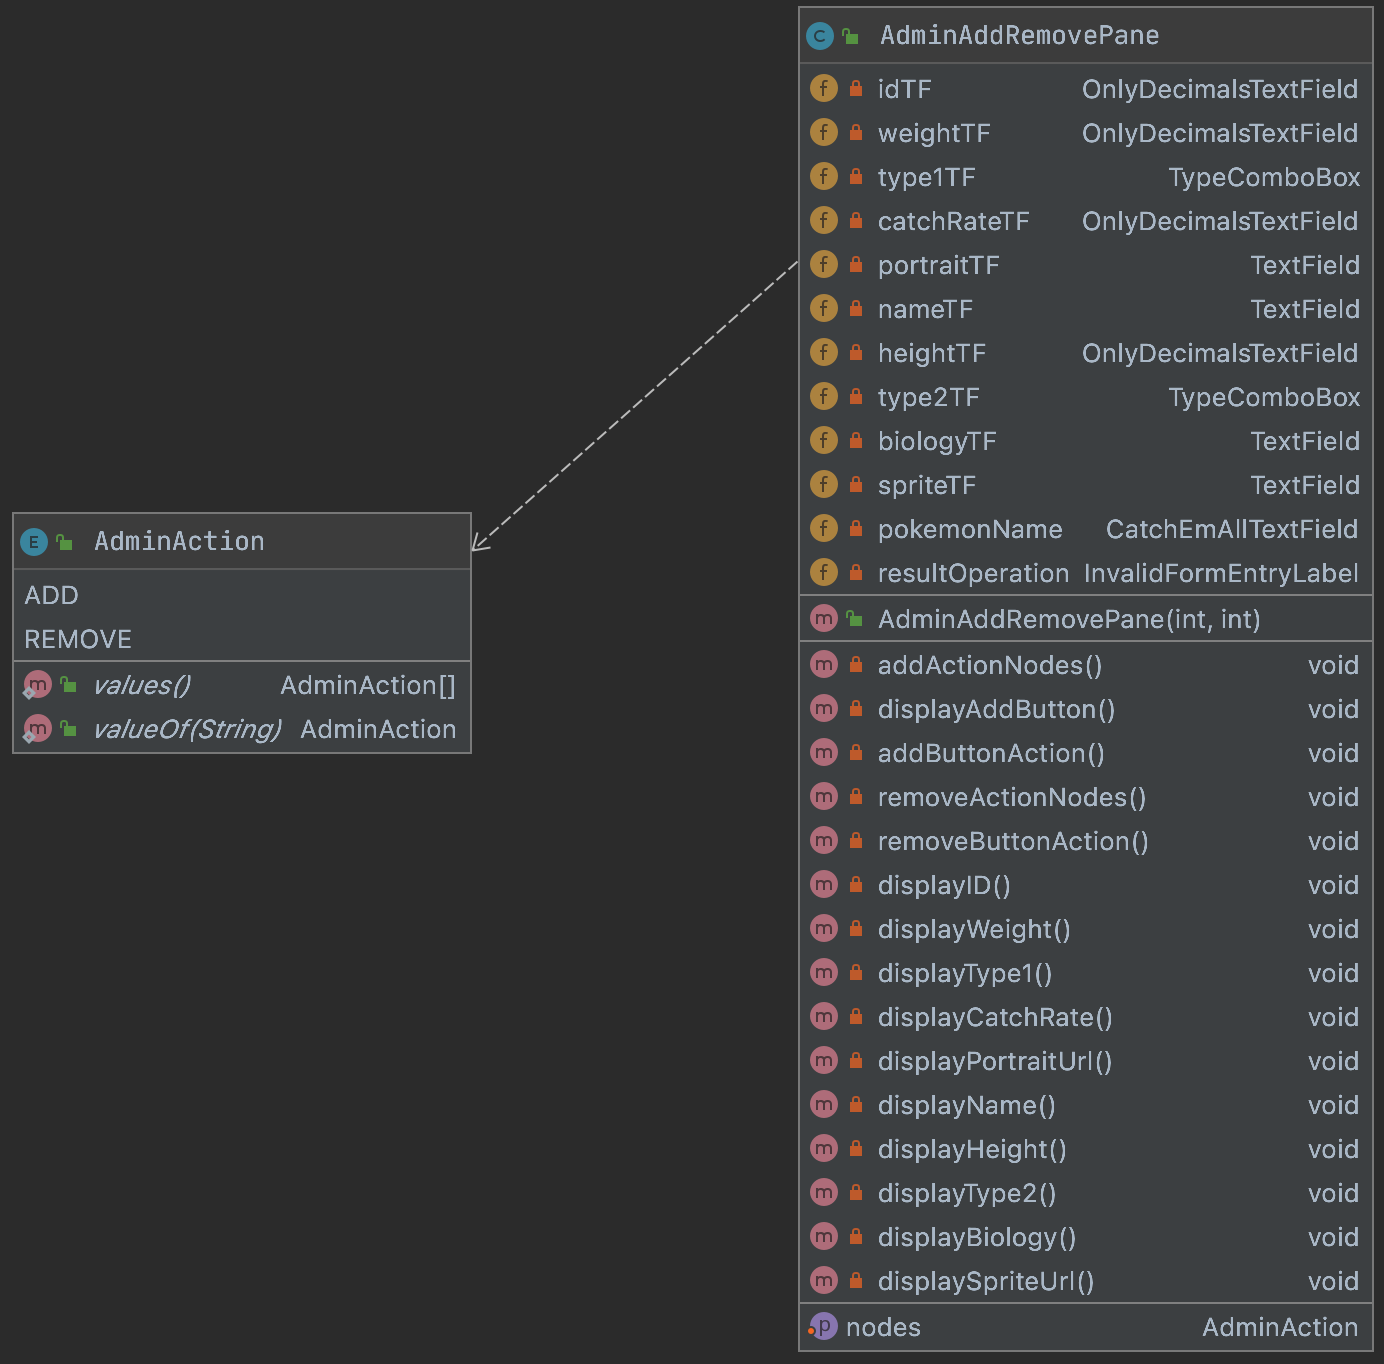
\includegraphics[width=0.7\textwidth]{img/javafx_panes_package3.png}
	\caption{javafxExtensions/panes/addRemove Package Class Structure}
\end{figure}

\begingroup
\setlength{\tabcolsep}{10pt} % Default value: 6pt
\renewcommand{\arraystretch}{1.5} % Default
\begin{center}
	\begin{longtable}{| m{14em} | m{19em} |} 
		\hline
		\textbf{Class Name} & \textbf{Short Description} \\ [0.5ex] 
		\hline
		AdminAddRemovePane & Specific Pane for the ADD/REMOVE scene.\\ 
		\hline
		AdminAction & Contains the name of the action that an admin can do regarding the \textbf{Pokèmon} management.\\ 
		\hline
	\end{longtable}
\end{center}
\endgroup


\subsubsection{Package Analysis: persistence}
The persistence package contains all the classes related to the communication with the databases. In the image below you can see how it is structured. The Factories classes are used as said before about the Ranking. 
\begin{figure}[H]
	\centering
	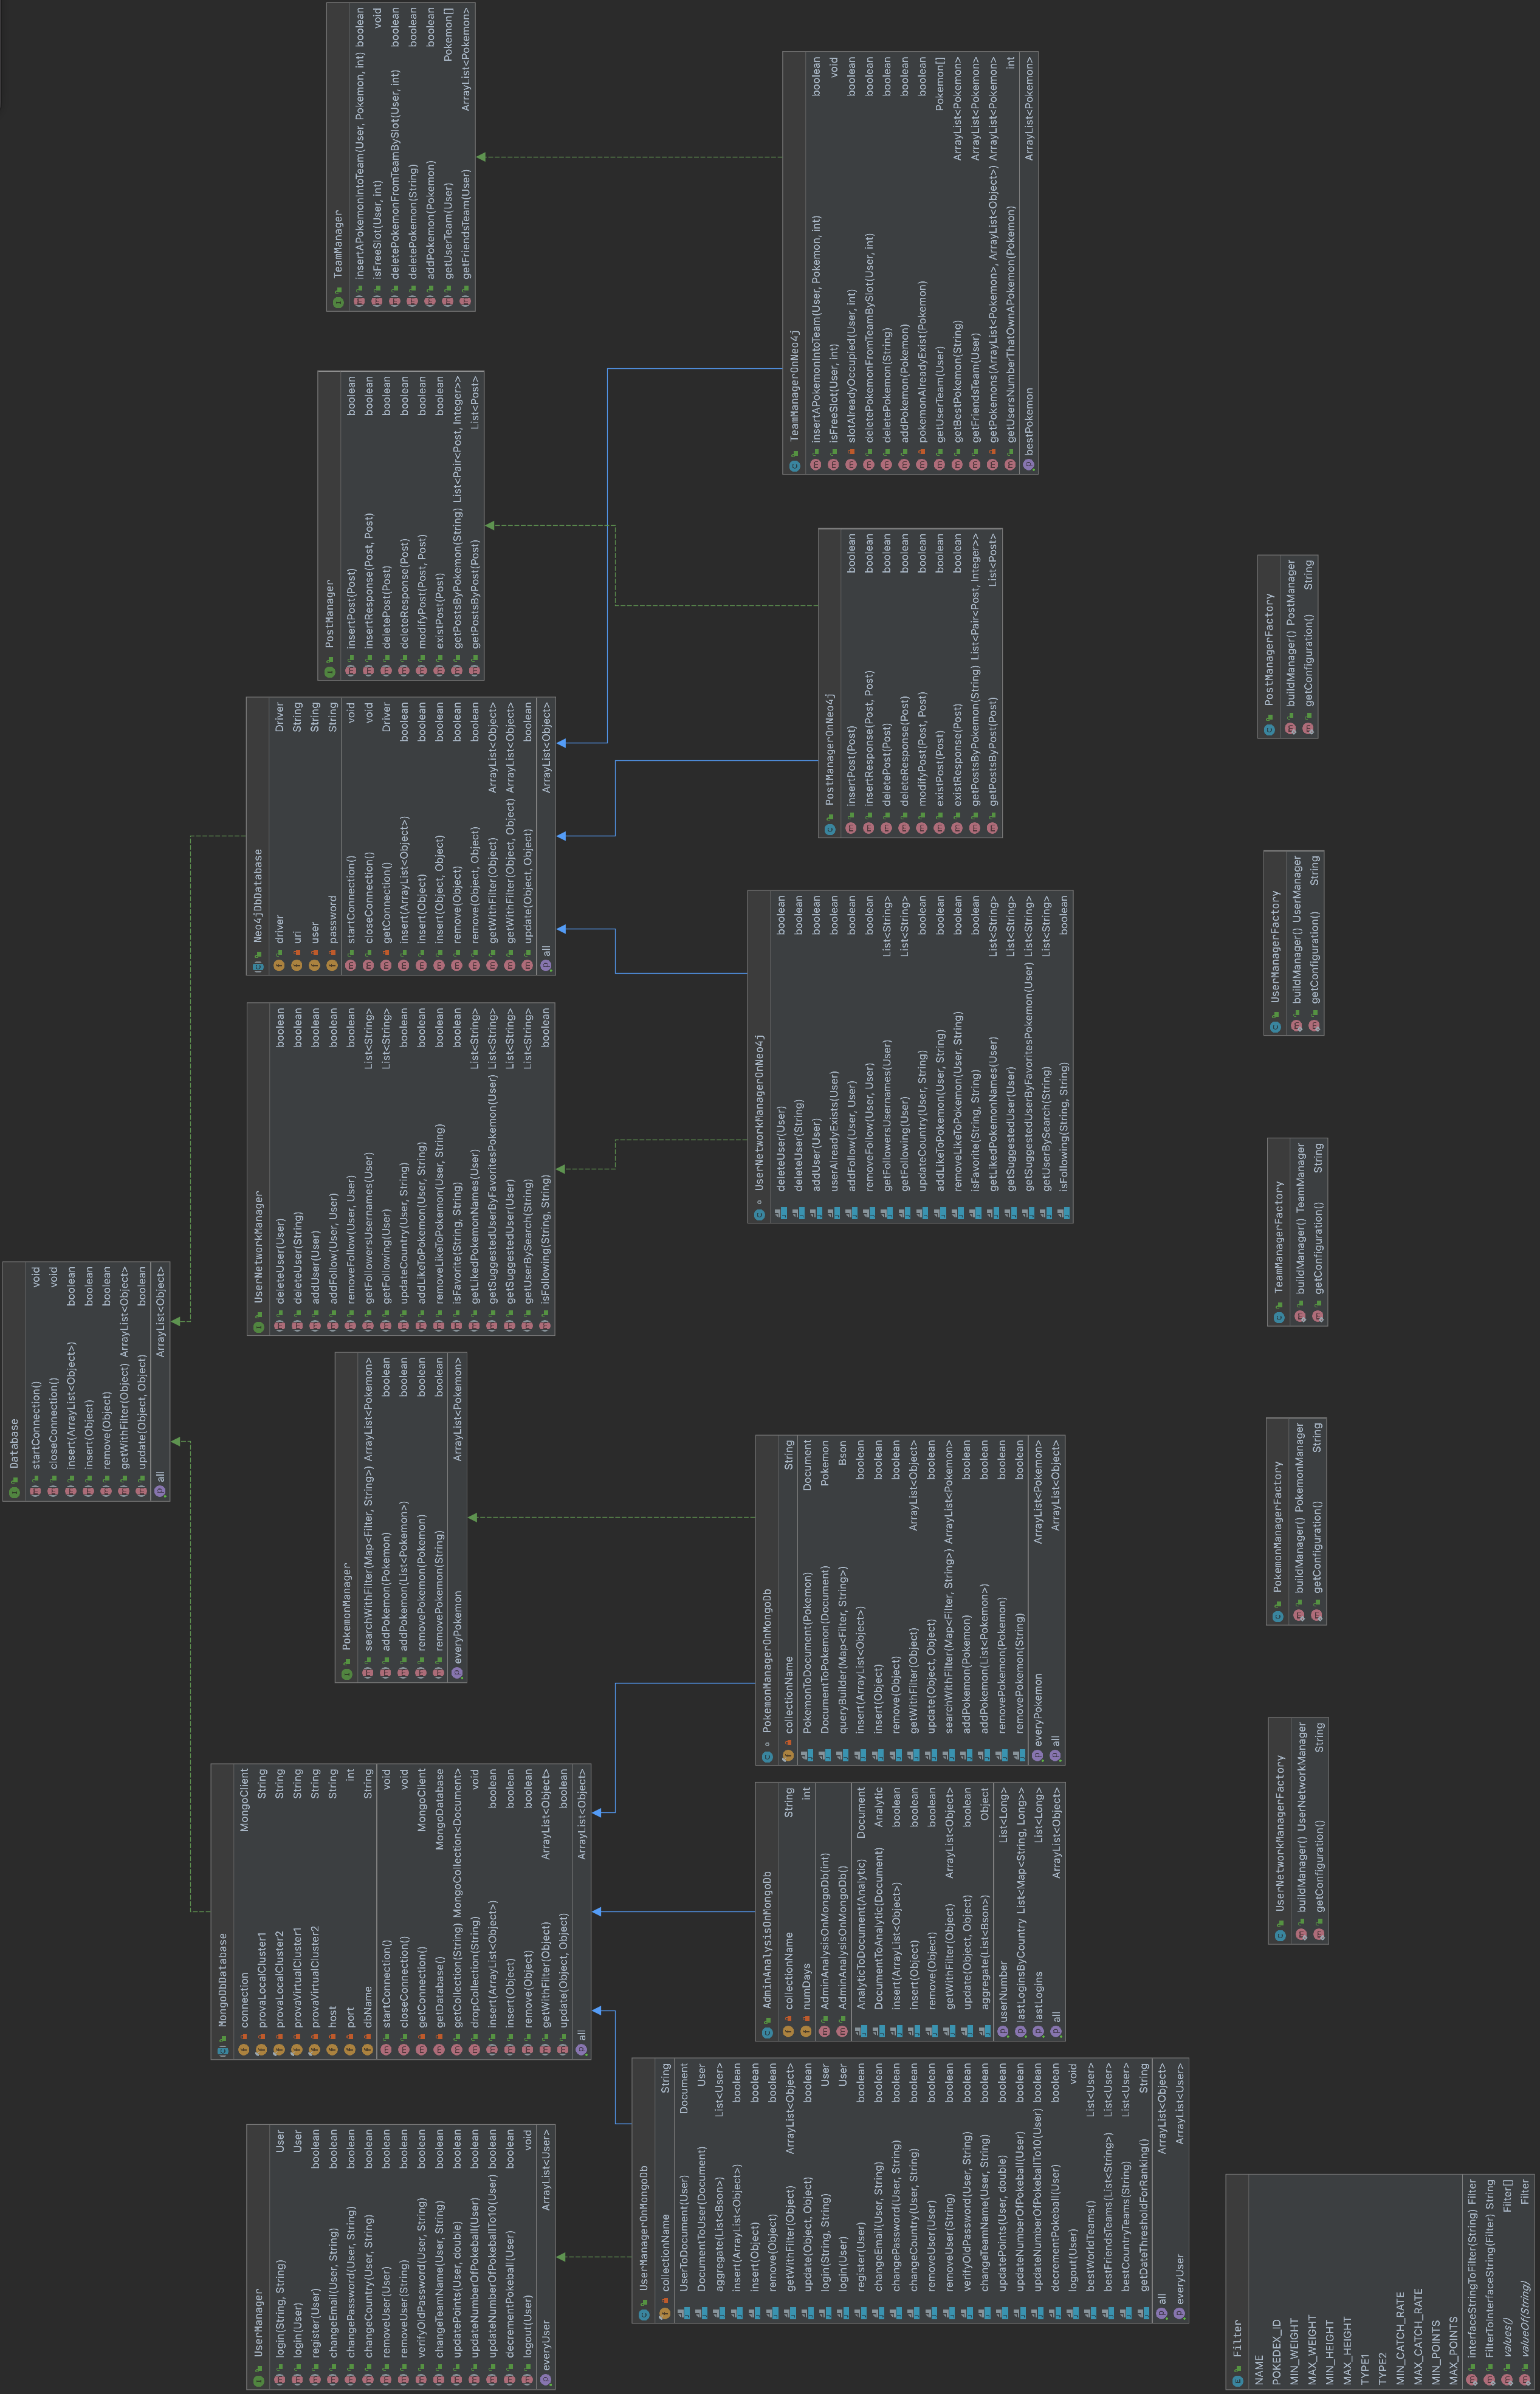
\includegraphics[width=0.9\textwidth]{img/persistence_package.png}
	\caption{persistence Package Class Structure}
\end{figure}

\begingroup
\setlength{\tabcolsep}{10pt} % Default value: 6pt
\renewcommand{\arraystretch}{1.5} % Default
\begin{center}
	\begin{longtable}{| m{14em} | m{19em} |} 
		\hline
		\textbf{Class Name} & \textbf{Short Description} \\ [0.5ex] 
		\hline
		Database & Shared interface among Databases, defines remote connections and structures of basic CRUD operations\\ 
		\hline
		UserManager & Shared interface for the managing of \textbf{Users}, defines the fundamental operations \\ 
		\hline
		PokemonManager & Shared interface for the managing of \textbf{Pokèmon}, defines the fundamental operations \\ 
		\hline
		UserNetworkManager & Shared interface for the managing of \textbf{Pokèmon}, defines the fundamental operations \\ 
		\hline
		PostManager & Shared interface for the managing of \textbf{Post}, defines the fundamental operations\\ 
		\hline
		MongoDbDatabase & Implementation of Database specific for MongoDB, to be extended with other classes.\\ 
		\hline
		UserManagerOnMongoDb & Extension of MongoDBDatabase, handles the \textbf{User} related queries in MongoDb\\ 
		\hline
		AdminAnalysisOnMongoDb & Extension of MongoDBDatabase, handles the admin related queries in MongoDb\\ 
		\hline
		PokemonManagerOnMongoDb & Extension of MongoDBDatabase, handles the \textbf{Pokèmon} related queries in MongoDb\\ 
		\hline
		Neo4jDbDatabase & Implementation of Database specific for Neo4j, to be extended with other classes.\\ 
		\hline
		UserNetworkManagerOnNeo4j & Extension of Neo4jDbDatabase, handles the \textbf{user} related queries in Neo4j\\ 
		\hline
		PostManagerOnNeo4j & Extension of Neo4jDbDatabase, handles the \textbf{Post} related queries in Neo4j\\
		\hline
		TeamManagerOnNeo4j & Extension of Neo4jDbDatabase, handles the \textbf{Team} related queries in Neo4j\\
		\hline
		Filter & Enum that contains the names of the filters used in the filter pane.\\
		\hline
		UserNetworkManagerFactory & Has a static method that returns a specific implementation of the interface UserNetworkManager\\
		\hline
		PokemonManagerFactory & Has a static method that returns a specific implementation of the interface PokemonManager\\
		\hline
		TeamManagerFactory & Has a static method that returns a specific implementation of the interface TeamManager.\\
		\hline
		UserManagerFactory & Has a static method that returns a specific implementation of the interface UserManager\\
		\hline
		PostManagerFactory & Has a static method that returns a specific implementation of the interface PostManager\\
		\hline
	\end{longtable}
\end{center}
\endgroup


\subsubsection{Package Analysis: security}
It contains the PasswordEncryptor class, we will discuss it in chapter 4.3.3

\subsubsection{Package Analysis: userInterface}
The userInterface package contains all the classes that are related to the creation of the GUI. The approach taken is a hierarchical one, in order to increase the modularity of the code.  
\begin{figure}[H]
	\centering
	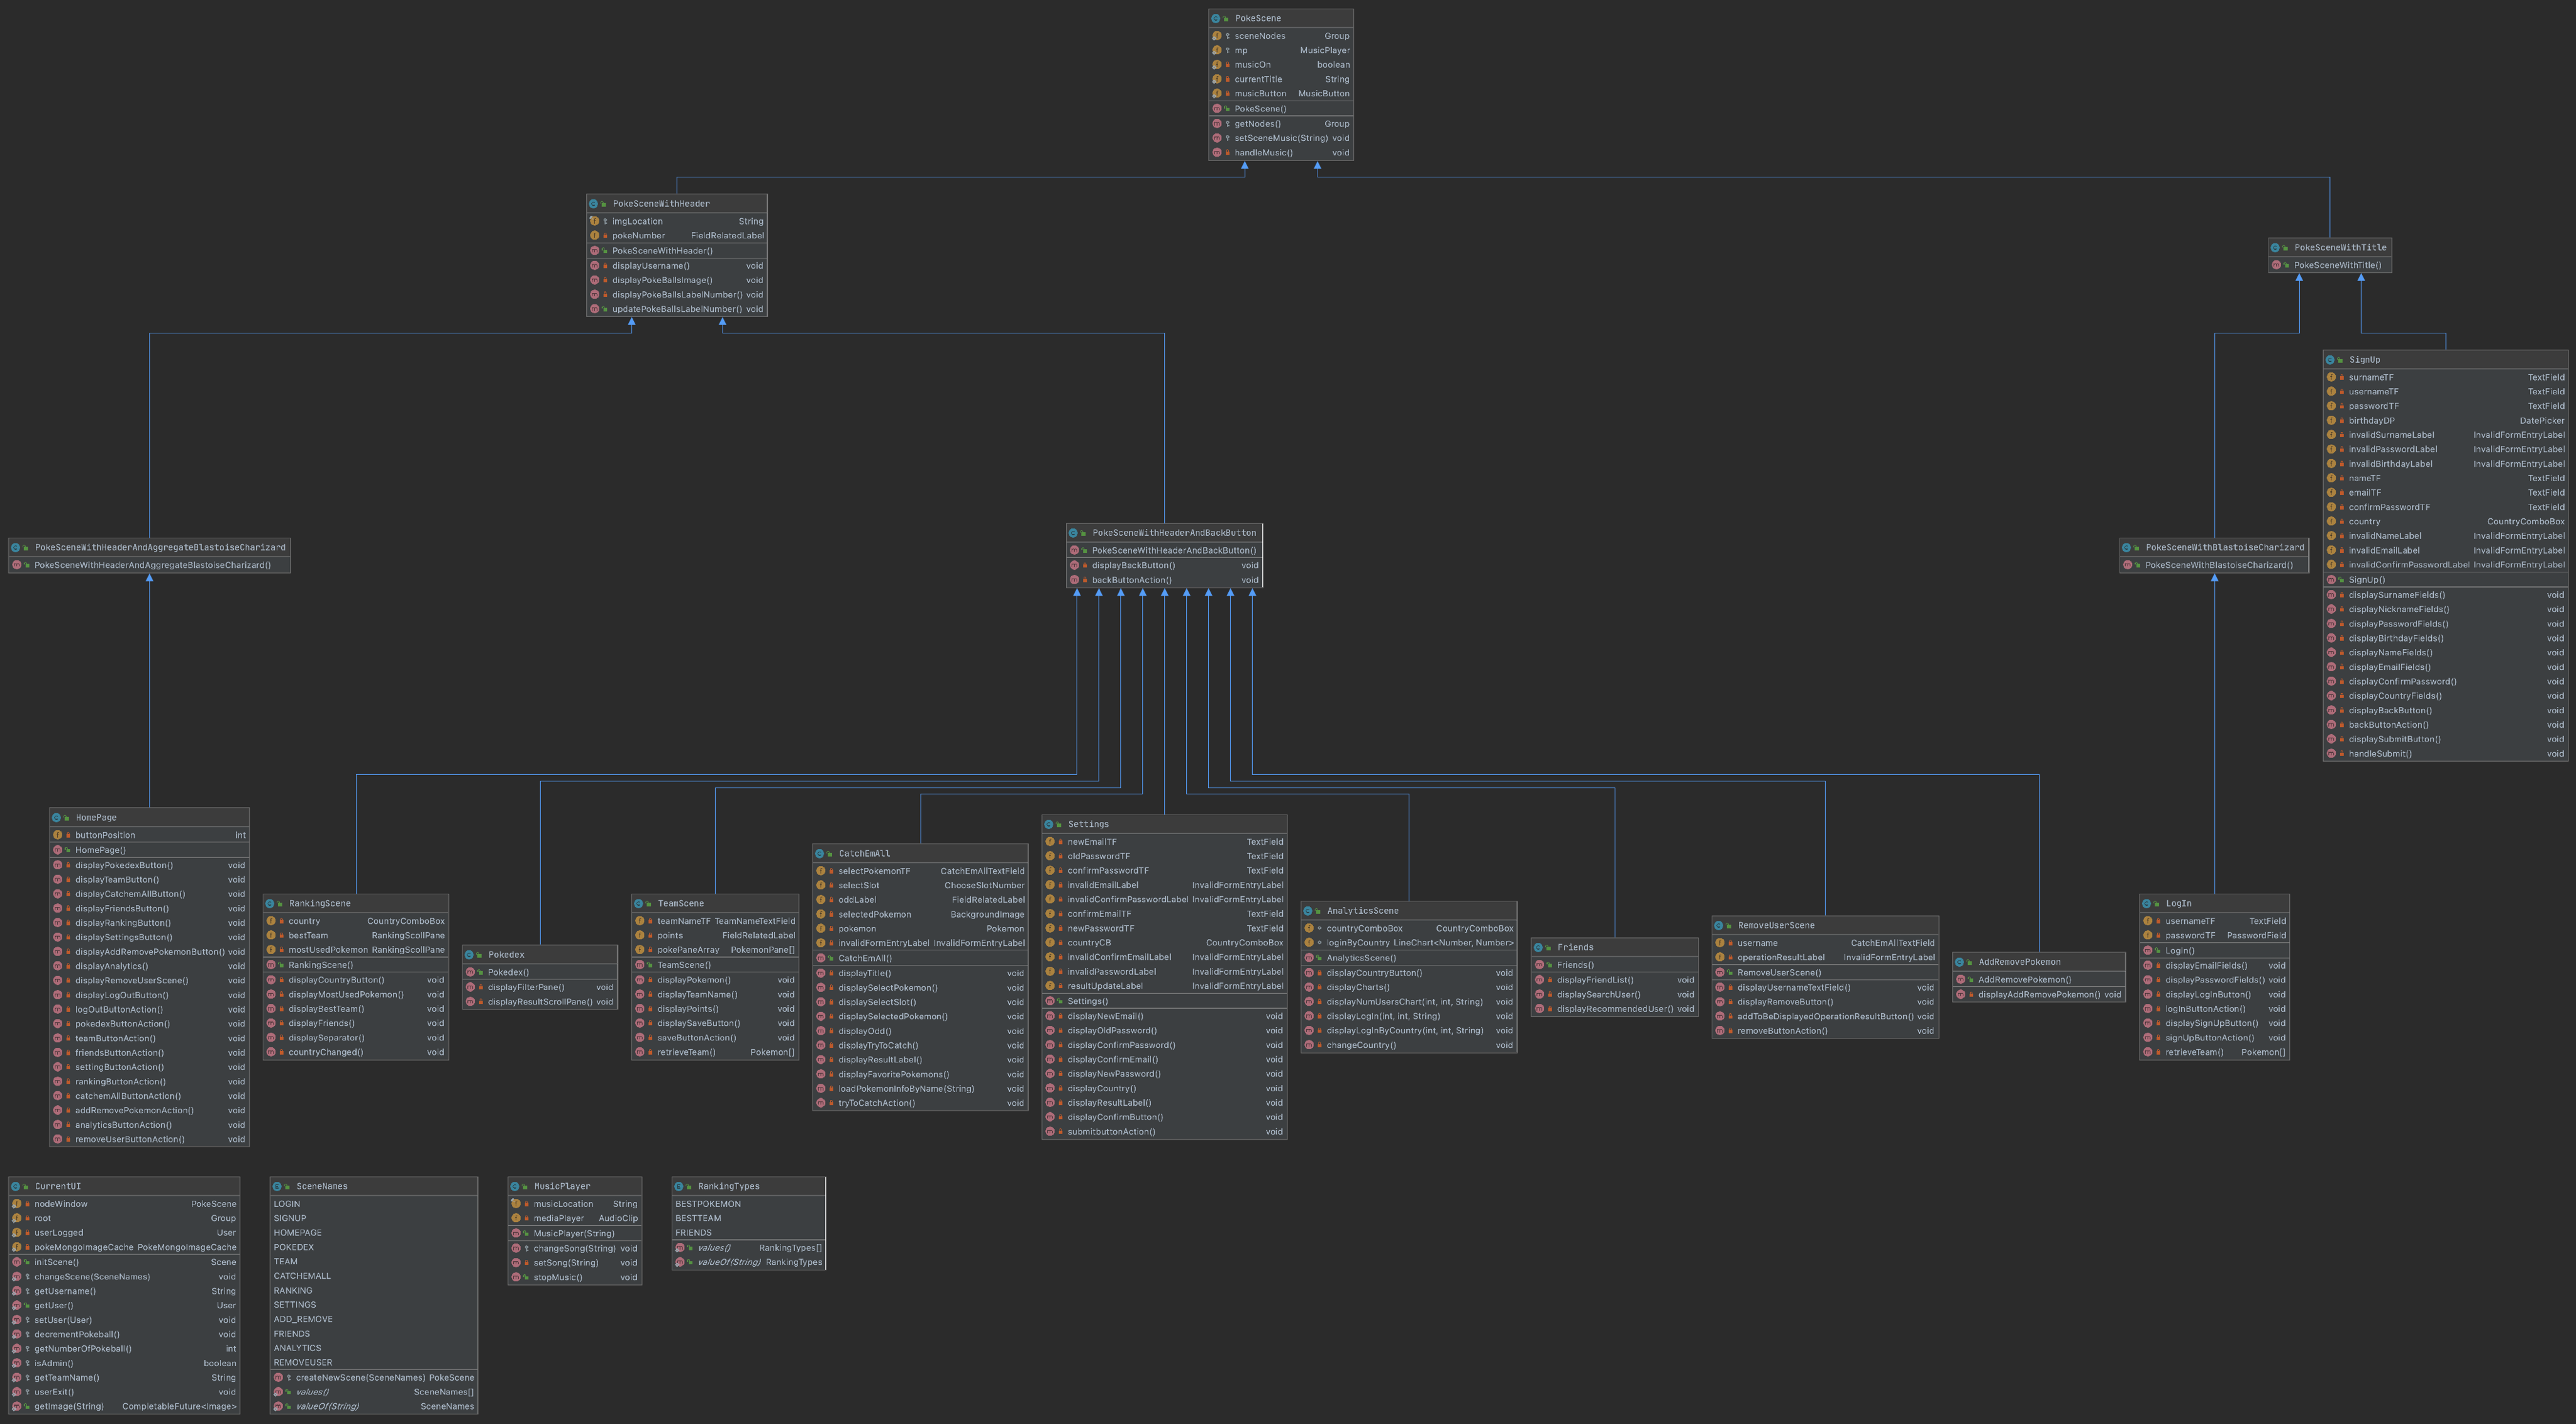
\includegraphics[width=\textwidth]{img/userInterface_package.png}
	\caption{userInterface Package Class Structure}
\end{figure}
\begingroup
\setlength{\tabcolsep}{10pt} % Default value: 6pt
\renewcommand{\arraystretch}{1.5} % Default
\begin{center}
	\begin{longtable}{| m{14em} | m{19em} |} 
		\hline
		\textbf{Class Name} & \textbf{Short Description} \\ [0.5ex] 
		\hline
		PokeScene & General scene that contains the elements shared by every scene\\ 
		\hline
		PokeSceneWithHeader & General scene with only the Header in it (the header contains the \textit{username} of the user logged and the number of \textbf{Pokèmon})\\ 
		\hline
		PokeSceneWithTitle & General scene with only the title\\ 
		\hline
		SignUp & Sign up page\\ 
		\hline
		PokeSceneWithBlastoise Charizard & General scene that extends PokeSceneWithTitle and adds to the scene the image of Charizard and Blastoise\\ 
		\hline
		LogIn & The first scene the user will see at the opening of the application. As the name suggests the class displays the Nodes regarding the LogIn\\ 
		\hline
		PokeSceneWithHeaderAnd AggregateBlastoiseCharizard & General scene that combines the PokeSceneWithHeader and the PokeSceneWithBlastoiseCharizard\\ 
		\hline
		HomePage & As the name suggests the class displays the Nodes regarding the HomePage\\ 
		\hline
		PokeSceneWithHeaderAndBack Button & General scene that contains the Header and the Back Button\\ 
		\hline
		RankingScene & As the name suggests the class displays the Nodes regarding the \textit{Ranking}\\ 
		\hline
		Pokedex & As the name suggests the class displays the Nodes regarding the \textit{Pokedex}\\ 
		\hline
		TeamScene & As the name suggests the class displays the Nodes regarding the \textbf{Team}\\
		\hline
		CatchEmAll & As the name suggests the class displays the Nodes regarding the \textit{CatchEmAll} page\\
		\hline
		Settings & As the name suggests the class displays the Nodes regarding the \textit{Settings}\\
		\hline
		AnalyticsScene & As the name suggests the class displays the Nodes regarding the \textit{Admin Analytics} scene\\
		\hline
		Friends & As the name suggests the class displays the Nodes regarding the \textit{Friends} scene\\
		\hline
		RemoveUserScene & As the name suggests the class displays the Nodes regarding the \textit{Remove User} scene\\
		\hline
		AddRemovePokemon & As the name suggests the class displays the Nodes regarding the scene where the admin can add or remove a \textbf{Pokèmon}\\
		\hline
		SceneNames & Enum containing the different types of scene. Helps for the managing the changing in the scenes.\\
		\hline
		RankingTypes & Enum containing the different types of ranking\\
		\hline
		MusicPlayer & Handles the music.\\
		\hline
		CurrentUI & Handles the current UI. This is the bone of the entire package.\\
		\hline
	\end{longtable}
\end{center}
\endgroup
\subsubsection{Package Analysis: utils}
This package contains utility classes. 
\begin{figure}[H]
	\centering
	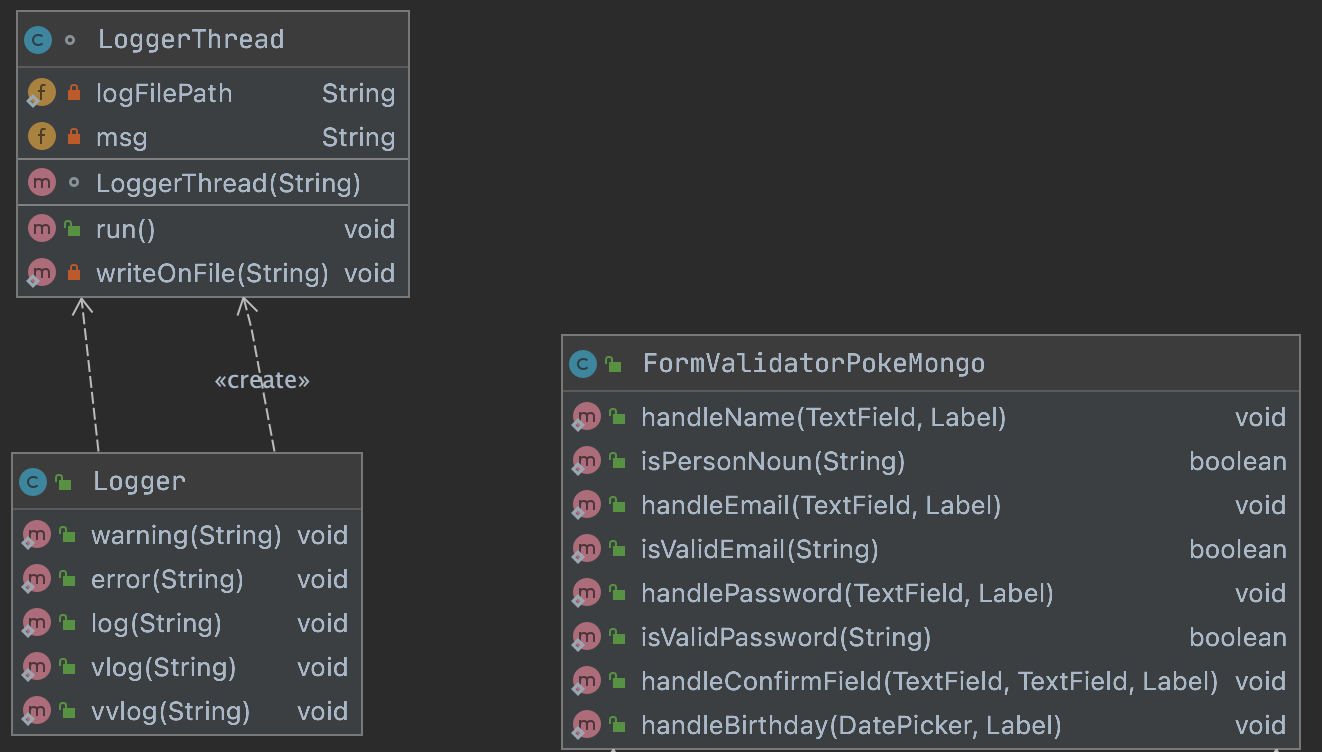
\includegraphics[width=0.7\textwidth]{img/utils_package.png}
	\caption{utils Package Class Structure}
\end{figure}
\begingroup
\setlength{\tabcolsep}{10pt} % Default value: 6pt
\renewcommand{\arraystretch}{1.5} % Default
\begin{center}
	\begin{longtable}{| m{14em} | m{19em} |} 
		\hline
		\textbf{Class Name} & \textbf{Short Description} \\ [0.5ex] 
		\hline
		FormValidatorPokeMongo & Used for check if a field is well filled\\ 
		\hline
		LoggerThread & A thread that writes information about all the action taken by the code.\\
		\hline
		Logger & Public logger that use the Thread one for handling all the logs.\\
		\hline
	\end{longtable}
\end{center}
\endgroup
Inside this package we added other two packages useful for the implementation of the initial data, thus they are not needed to the user that uses the application (in a possible publish this part will be erased).\\
The \textbf{autoLog} packages contains a java file named \textit{AutoLogin}:
\begin{lstlisting}[language=Java]
	public class AutoLogIn {
		public static void main(String[] args) {
			// TAKE ALL THE USERS
			UserManager userManager = UserManagerFactory.buildManager();
			ArrayList<User> allUsers = userManager.getEveryUser();
			
			for (User user: allUsers) {
				if (Math.random() < .7)
				continue;
				userManager.login(user.getUsername(),user.getName() + user.getSurname() + "000");
				
				user.addTeam(retrieveTeam(user));
				
				// Update the point in mongodb
				userManager.updatePoints(user, user.getPoints());
			}
		}
		
		private static Pokemon[] retrieveTeam(User user) {
			TeamManager teamManager = TeamManagerFactory.buildManager();
			return teamManager.getUserTeam(user);
		}
	}
	
\end{lstlisting}

The main method retrieves all the user from the db and for each of them calculate a value using Math.random(). If this value is less than 0.7 the for loop continues with the next iteration (this is not for waiting not too many hours). If the if turn out to be true, we login in in the \textbf{User} account, we retrieve his/her \textbf{Team} and then we calculate and update the points.\\
This class comes in handy for generating some useful data by our own.

The \textbf{dbPopulators} package contains a java file named \textit{UserPopulator}. This class has a main method that creates randomly users to be added in MongoDb (as described in chapter 2.3). What it does is picking a random name, surname and country from the related txt files and some other random information that are required for registering and instantiates a new User object, that is stored in the db by a specific database method.

\subsubsection{APIs and SPIs}
In the package named \textit{persistence} we, for the sake of code obfuscation (as told 4.1.1), created a API/SPI relation. The main Service Provider Interface is the class Database that defines remote connections and structures of basic CRUD operations. Here a look up:

\begin{lstlisting}[language=Java]
	/**
	* starts the connection with the remote Database
	*/
	void startConnection();
	
	/**
	* closes the connection with the remote Database
	*/
	void closeConnection();
	
	
	/**
	* insert 1 ore more objects into the database
	* @param toInsert ArrayList of arbitrary objects to insert into the Database
	* @return true if at least one element has been added
	*/
	boolean insert(ArrayList<Object> toInsert);
	
	/**
	* insert 1 object into the database
	* @param toInsert ArrayList of arbitrary objects to insert into the Database
	* @return true if exactly one element has been added
	*/
	boolean insert(Object toInsert);
	
	/**
	* remove 1 ore more objects from the database
	* @param o is an Object to remove or a query to submit
	* @return true if at least one element has been removed
	*/
	boolean remove(Object o);
	
	/**
	* gets all the elements
	* @return a list of retrieved elements
	*/
	ArrayList<Object> getAll();
	
	/**
	*
	* @param filter query or filter to submit to the db
	* @return a list of retrieved elements
	*/
	ArrayList<Object> getWithFilter(Object filter);
	
	/**
	*
	* @param target query or object to update
	* @param newValue new value for the target
	* @return true if at least one object is updated
	*/
	boolean update(Object target, Object newValue);
}
\end{lstlisting}
From this interface we created different implementations, one for every database used, which are \textit{Neo4jDbDatabase} and \textit{MongoDbDatabase}. Although, this two classes are abstract, thus they are extended for creating query specific private classes (e.g., \textit{PokemonManagerOnMongoDb} handles all the query related to \textbf{Pokémon} on MongoDb).
For making use of those private classes, we have to use some APIs called Factory. We have a factory for each query specific class type:

\begingroup
\setlength{\tabcolsep}{10pt} % Default value: 6pt
\renewcommand{\arraystretch}{1.5} % Default
\begin{center}
	\begin{longtable}{| m{16em} | m{16em} |} 
		\hline
		\textbf{Query Specific Type} & \textbf{Factory} \\ [0.5ex] 
		\hline
		Managing \textbf{Pokèmon} & PokemonManagerFactory\\ 
		\hline
		Managing \textbf{Post} & PostManagerFactory\\
		\hline
		Managing \textbf{Team} & TeamManagerFactory\\
		\hline
		Managing \textbf{User} information & UserManagerFactory\\
		\hline
		Managing the network between \textbf{Users} & UserNetworkManagerFactory\\
		\hline
	\end{longtable}
\end{center}
\endgroup

Every query specific type has also an own interface that works as SPI.
The structure of a factory class is the following, here the \textit{PokemonManagerFactory}:

\begin{lstlisting}[language=Java]
	public class PokemonManagerFactory {
		public static PokemonManager buildManager(){
			String technology = getConfiguration();
			Logger.vlog("Obtaining technology: " + technology);
			switch (technology){
				case "MongoDb":
				return new PokemonManagerOnMongoDb();
				default:
				try{
					throw new IllegalArgumentException();
				}catch (IllegalArgumentException iae){
					iae.printStackTrace();
					Logger.error("Invalid database technology or missing implementation");
				};
				return null;
			}
		}
		
		public static String getConfiguration(){
			return ConfigDataHandler.getInstance().configData.pokemonDbArchitecture;
		}
	}
\end{lstlisting}

What it actually does is checking the configuration technology, retrieved that, it switches in order to use the one requested. If it’s one of the presented in the case period then it will retrieve the appropriate class object, otherwise it will throw an exception.

\subsubsection{Obfuscation}
Our package structure organization gave us the possibility to exploit code obfuscation. We use code obfuscation in the way to hide how the connection of the database is done. To do that we limited some classes to have only a package scope and, to interact with them, we use the Manager classes presented before.

%\subsection{APIs and SPIs}

\subsection{Main tools}
For enhancing our performances and for giving to the user a better application, some tool are used. We focus in this chapter about: GSON, caching system, password encrypt and the logger.
\subsubsection{GSON}
Gson is a Java library that can be used to convert Java Objects into their JSON representation. It can also be used to convert a JSON string to an equivalent Java object. Gson can work with arbitrary Java objects including pre-existing objects that you do not have source-code of.
We use Gson mainly for communicating with MongoDb and for setting the configuration information.
\subsubsection{Caching mechanism and multimedia management}
The Pokemon game series became famous for the creature a player can capture and use, so we thought to include the \textbf{Pokèmon} images also in our project.\\
The images about the \textbf{Pokèmons} are not stored locally, because this will increase our project size too much. To avoid this huge increment we take all the images, only when they are needed, from a GitHub repository. Here a problem came: loading a lot of images would slow down our system and that is against our no-functional requirements. The caching comes then in handy.

\begin{lstlisting}[language=Java]
	public class PokeMongoImageCache implements PokeMongoCache {
		//Singleton
		private static PokeMongoImageCache instance;
		private AsyncLoadingCache<String, Image> cache;
		
		public static PokeMongoImageCache getInstance() {
			if (instance == null) {
				instance = new PokeMongoImageCache();
			}
			return instance;
		}
		
		PokeMongoImageCache(){
			cache = Caffeine.newBuilder()
			.expireAfterAccess(10, TimeUnit.MINUTES) 
			.maximumSize(1000) 
			.buildAsync(k -> PokemonImage.get(k));
		}
		
		public CompletableFuture<Image> getDataIfPresent(String url){
			Logger.vlog("Attemp to get image at: " + url);
			return cache.get(url);
		}
	}
\end{lstlisting}

What the cache does is simply store asynchronously an image. Why asynchronous? If the operation would be done in a synchronous way the user has to wait that the image is properly store for seeing and using the UI. Using an asynchronous way the user can interact with the UI even if the images are already loaded, this create a better application usage.
\subsubsection{Password Encryptor}
Encrypting a password is typically used to protect it from eavesdropping. We encrypt it and then we sent it to the database, in this way no eavesdropper can snatch the password in transit.
How does the encryption is done? We decided to use the class org.apache.commons.codec.digest.DigestUtils, that has operations to simplify common MessageDigest tasks. Thus, we use DigestUtils.sha256Hex() calculate the SHA-256 digest of a string composed by the password of the user plus one other string.

\begin{lstlisting}[language=Java]
	public class PasswordEncryptor {
		
		@VisibleForTesting
		public static String encryptPassword(String plainPassword){
			String s = "randomSalt";
			String encryptedPassword = cipher(plainPassword, s);
			return encryptedPassword;
		}
		
		public static String cipher(String pwd, String salt) {
			return DigestUtils.sha256Hex(pwd+salt);
		}
	}
\end{lstlisting}
\subsubsection{Logger}
We thought that useful logs would provide us (especially when someone has to debug/maintain someone else’s code) with help when trying to understand what the code actually does. The Logger takes care of recording the events that happen during runtime.
\begin{lstlisting}[language=Java]
	public class Logger {
		
		public static void warning(String text){
			if(ConfigDataHandler.getInstance().configData.verbosityLevel >= 1){
				LoggerThread lt = new LoggerThread("[WARNING] " + text);
				lt.start();
			}
			
		}
		
		public static void error(String text){
			if(ConfigDataHandler.getInstance().configData.verbosityLevel >= 1){
				LoggerThread lt = new LoggerThread("[ERROR] " + text);
				lt.start();
			}
		}
		
		public static void log(String text){
			if(ConfigDataHandler.getInstance().configData.verbosityLevel >= 1){
				LoggerThread lt = new LoggerThread("[LOG] " + text);
				lt.start();
			}
		}
		
		public static void vlog(String text){
			if(ConfigDataHandler.getInstance().configData.verbosityLevel >= 2){
				LoggerThread lt = new LoggerThread("[VLOG] " + text);
				lt.start();
			}
		}
		
		public static void vvlog(String text){
			if(ConfigDataHandler.getInstance().configData.verbosityLevel >= 3){
				LoggerThread lt = new LoggerThread("[VVLOG] " + text);
				lt.start();
			}
		}
	}
\end{lstlisting}

Every function create and start a new LoggerThread, it will simply print in a file the log infos.

\begin{lstlisting}[language=Java]
	class LoggerThread extends Thread{
		private static String logFilePath="log/logFile.txt";
		private String msg;
		
		LoggerThread(String msg){
			this.msg=msg;
		}
		
		public void run(){
			String newMsg = Instant.now().toString() + " " + msg + "\n";
			writeOnFile(newMsg);
		}
		
		private static synchronized void writeOnFile(String msg){
			try {
				Files.write(Paths.get(logFilePath), msg.getBytes(), StandardOpenOption.APPEND);
			}
			catch (IOException i){
				i.printStackTrace();
			}
		}
		
	}
\end{lstlisting}

\subsubsection{Form Validator}
The FormValidatorpokMongo checks if the \textbf{User} fills the textfields in the proper way, if he doesn’t that it shows up an error as a label. The validator functions makes use of Regular Expression, in this way me ensure that the field is well written.
\begin{lstlisting}[language=Java]
	public class FormValidatorPokeMongo {
		
		/**
		* In this section are present the event handler for the 'setOnKeyReleased' event in the form.
		*/
		public static void handleName(TextField nameTF, Label invalidNameLabel){
			if(FormValidatorPokeMongo.isPersonNoun(nameTF.getText()))
			invalidNameLabel.setVisible(false);
			else
			invalidNameLabel.setVisible(true);
		}
		
		/**
		* Check if the string contains only letters, spaces, dots and apostrophes.
		*/
		@VisibleForTesting
		public static boolean isPersonNoun(String possibleNoun){
			Pattern pattern = Pattern.compile("^[a-zA-Z '.]+$");
			Matcher matcher = pattern.matcher(possibleNoun);
			return matcher.find();
		}
		
		public static void handleEmail(TextField emailTF, Label invalidEmailLabel){
			if(FormValidatorPokeMongo.isValidEmail(emailTF.getText()))
			invalidEmailLabel.setVisible(false);
			else
			invalidEmailLabel.setVisible(true);
		}
		
		/**
		* Check if the email follows the format example@domain.tld
		*/
		@VisibleForTesting
		public static boolean isValidEmail(String possibleEmail){
			Pattern pattern = Pattern.compile("^[\\w-\\.]+@([\\w-]+\\.)+[\\w-]{2,4}$");
			Matcher matcher = pattern.matcher(possibleEmail);
			return matcher.find();
		}
		
		public static void handlePassword(TextField passwordTF, Label invalidPasswordLabel){
			if(FormValidatorPokeMongo.isValidPassword(passwordTF.getText()))
			invalidPasswordLabel.setVisible(false);
			else
			invalidPasswordLabel.setVisible(true);
		}
		
		/**
		* Checks if the password contains minimum eight characters, at least one letter and one number.
		*/
		@VisibleForTesting
		public static boolean isValidPassword(String possiblePassword){
			Pattern pattern = Pattern.compile("^(?=.*[A-Za-z])(?=.*\\d)[A-Za-z\\d]{8,}$");
			Matcher matcher = pattern.matcher(possiblePassword);
			return matcher.find();
		}
		
		public static void handleConfirmField(TextField fieldTF, TextField confirmFieldTF, Label invalidConfirmFieldLabel){
			String password = fieldTF.getText(), confirmPassword = confirmFieldTF.getText();
			
			if(password.equals(confirmPassword))
			invalidConfirmFieldLabel.setVisible(false);
			else
			invalidConfirmFieldLabel.setVisible(true);
		}
		
		/**
		* Checks if the birthday date selected is valid: future dates cannot be picked
		*/
		public static void handleBirthday(DatePicker birthdayDP, Label invalidBirthdayLabel){
			LocalDate localDate = birthdayDP.getValue();
			LocalDate today = LocalDate.now();
			System.out.println(today);
			
			if(localDate.isAfter(today)){
				invalidBirthdayLabel.setVisible(true);
			} else {
				invalidBirthdayLabel.setVisible(false);
			}
		}
	}
\end{lstlisting}

\subsection{Business Logic}
The business logic used in \textbf{\textit{PokeMongo}} is the following. To ensure a high variability between \textbf{Teams} we decided to cope the \textit{catch rate} of each \textbf{Pokemon} in a way that if it is held by a lot of \textbf{Users} it will decrease, thus will let \textbf{Users} to try to catch other \textbf{Pokemon}, with the same rarity but held by less people. Although, the \textit{catch rate} is related also to the \textit{points}, if a \textbf{Pokemon} has a lower \textit{catch rate} the \textit{points} are higher, so catching other \textbf{Pokemon} (not the famous ones) may look like illogical at first, but keep in mind that the probability that having a rare \textbf{Pokemon} is very low as the “CATCH’EM ALL” page, so it is quite impossible that every user has the same rare \textbf{Pokemons}.
\subsubsection{Points computing}
The \textit{points} related to a \textbf{Pokemon} are computed in a very simple way and they are strictly linked to the catch rate of a \textbf{Pokèmon} (a value between 3 and 255).
\begin{equation}
	points_{single\ pokemon} = 255 - dynamic\ catch\ rate 
\end{equation}
The total \textit{points} held by a \textbf{User} is computed as follow:
\begin{equation}
	Total\ points=\left(\sum_{Team}{points}_{single\ pokemon}\right)\times{multiplier}
\end{equation}
The multiplier is a value of 1.5 that is applied when in the\textbf{ \textbf{Team} are presented all Pokemon that has different types} from each other, otherwise the multiplier will be 1.
The total points is computed only when a \textbf{User} login or when he catches/remove a \textbf{Pokèmon}.

\subsubsection{Dynamic Catch Rate computing}
The\textbf{ dynamic catch rate} is expatiate as follows:

\begin{equation}
	dyn.\ catch\ rate= catch\ rate \times \left(1-\frac{\# users\ that\ has\ the\ Pokemon}{total\ number\ of\ users}\right)
\end{equation}


\subsection{MongoDB: Analytics queries implementation}
In this chapter are present how the analytic queries are computed by exploiting the MongoDB database.

\subsubsection{User Rankings}
We have three different types of ranking that regards the \textbf{Users}: the \textit{World Best Team}, the \textit{Friend Best Team} and the \textit{“Country” Ranking} (where \textit{country} is a specific country, e.g. Italy).
\paragraph{World Best Team}
The \textit{World Best Team} consider all the \textbf{User} in the world and retrieve a limited number of \textbf{User} who has the highest value of \textit{points}. This is done querying MongoDb as follow:

\begin{comment}
\begin{lstlisting}[language=Java]
	public List<User> bestWorldTeams() {
		Bson match = match(and(eq("admin", false), lte("lastLogin", getDateThresholdForRanking())));
		Bson sort = sort(descending("points", "birthDay"));
		Bson limit = limit(ConfigDataHandler.getInstance().configData.numRowsRanking);
		Bson project = project(fields(excludeId(), include("username", "teamName", "points", "birthDay", "country")));
		return aggregate(Arrays.asList(match, sort, limit, project));
	}
\end{lstlisting}
\end{comment}

\begin{lstlisting}[language=Java]
	db.user.aggregate([
		{$match: {"admin": {$eq: false}, "lastLogin": {$lte: $tresholdDate}}},
		{$sort: {"points": -1, "birthDay": -1}},
		{$limit: $limitNum},
		{$project: {"_id": 0, "username": 1, "teamName": 1, "birthDay":1, "country": 1}}
	]);
\end{lstlisting}

What is done is matching \textbf{Users} that aren’t admin and that have the \textit{lastLogin} field within a certain range of days. Then we order the result in a descending way, considering the \textit{points} and the birth day, this one just to order \textbf{Users} that have the same value for \textit{points} in order to greeting younger players. As said before we limit the number of result (this can be modified in the configuration file) and we project only the feature we are interested into.\\
We have limited the ranking based on \textit{lastLogin}, because the \textbf{User} \textit{points} are only updated when the \textbf{User} use the application,  in order to have a less computational effort in the server databases. This, also, makes the \textbf{User} \textit{points} something that \textbf{lose meaning after a certain period of time}.

\paragraph{Friends Best Team}
After obtaining friends \textit{usernames} on Neo4j we compute:
\begin{lstlisting}[language=Java]
	db.user.aggregate([
	{$match: {"admin": {$eq: false}, "lastLogin": {$lte: $tresholdDate, "username": {$in: $friendsUsernames}}}},
	{$sort: {"points": -1, "birthDay": -1}},
	{$limit: $limitNum},
	{$project: {"_id": 0, "username": 1, "teamName": 1, "birthDay":1, "country": 1}}
	]);
\end{lstlisting}
\paragraph{Country Best Team}
This is similar to the \textit{World Best Team}, but we use an additional match for the country.

\begin{comment}
\begin{lstlisting}[language=Java]
	public List<User> bestCountryTeams(String country) {
	Bson match = match(and(eq("country", country), eq("admin", false), lte("lastLogin", getDateThresholdForRanking())));
	Bson sort = sort(descending("points", "birthDay"));
	Bson project = project(fields(excludeId(), include("username", "teamName", "points", "birthDay", "country")));
	Bson limit = limit(ConfigDataHandler.getInstance().configData.numRowsRanking);
	return aggregate(Arrays.asList(match, sort, limit, project));
	}
\end{lstlisting}
\end{comment}

\begin{lstlisting}[language=Java]
	db.user.aggregate([
		{$match: {"country": $country, "admin": {$eq: false}, "lastLogin": {$lte: $tresholdDate}}},
		{$sort: {"points": -1}},
		{$limit: $limitNum},
		{$project: {"_id": 0, "username": 1, "teamName": 1, "birthDay":1, "country": 1}}
	]);
\end{lstlisting}




\subsubsection{Usage Statistics}
We created few function for handling some simple statistics that can be useful for the \textbf{admin User}, in order to see how many the people in the world use the application and how often. We decided to include three types of statistic: \textit{total number of users}, \textit{users that logged during a single day}, \textit{users that logged during a single day in a specific country}. Because all the information needed is stored in MongoDb we query the database in order to create a new document with all the information specific for the analytics of a single day.

\paragraph{Total Users}:
\begin{lstlisting}[language=Java]
	db.user.aggregate([
		{$match: {"admin": {$eq: false}}},
		{$group: {_id: "admin", "userNumber": {$sum: 1}}},
		{$project: {"_id": 0, "userNumber": 1}}
	]);
\end{lstlisting}
\paragraph{Today Login}:
\begin{lstlisting}[language=Java]
	db.user.aggregate([
		{$match: {"lastLogin": {$gte: $yesterdayDate}, "admin": {$eq: false}}},
		{$group: {_id: "admin", "userNumber": {$sum: 1}}},
		{$project: {"_id": 0, "userNumber": 1}}
	]);
\end{lstlisting}
\paragraph{Country Today Login}:
\begin{lstlisting}[language=Java]
	db.user.aggregate([
		{$match: {"lastLogin": {$gte: $yesterdayDate}, "admin": {$eq: false}}},
		{$group: {_id: "country", "lastLogin": {$sum: 1}}},
		{$sort: {"lastLogin": -1}},
		{$project: {"_id": 1, "lastLogin": 1}}
	]);
\end{lstlisting}
\subsection{Neo4j: Recommendation and main queries implementation}

\paragraph{Best Pokemon by Country}: Return \textbf{Pokèmon} most captured by \textit{country}:
\begin{lstlisting}[language=SQL]
	MATCH (u:User)-[h:HAS]->(p:Pokemon) 
	WHERE u.country = $country return p.name, count(h) AS held, p.sprite 
	ORDER BY held 
	DESC LIMIT
\end{lstlisting}

\paragraph{Delete User}: Delele a \textbf{User} from Neo4j Database. Also all the posts/replies written by that \textbf{User} (and the related replies) will be removed. 
\begin{lstlisting}[language=SQL]
	MATCH (u:User) WHERE u.username = $username 
	OPTIONAL MATCH (u)-[:CREATED]->(p:Post)
	OPTIONAL MATCH (p)<-[:TOPIC]-(p1:Post)
	DETACH DELETE u, p, p1
\end{lstlisting}

\paragraph{Delete Pokemon}: Delele a \textbf{Pokèmon} from Neo4j Database. Also all the posts and replies regarding that \textbf{Pokèmon} will be removed. 
\begin{lstlisting}[language=SQL]
	MATCH (p:Pokemon) WHERE p.name = $name
	OPTIONAL MATCH (p:Pokemon)<-[:TOPIC]-(pp:Post)<-[:TOPIC]-(pp1:Post) 
	DETACH DELETE p, pp, pp1
\end{lstlisting}

\paragraph{Friends Recommendation by Followers}: friends recommended by followers (friends) are all the different \textit{followers of the followers} of the \textbf{User} (an already followed \textbf{User} is not returned).
\begin{lstlisting}[language=SQL]
	MATCH (u:User)-[:FOLLOW]->(u1:User)-[:FOLLOW]->(u2:User) 
	WHERE NOT (u)-[:FOLLOW]->(u2) and u2 <> u and u.username = $username 
	RETURN u2.username 
	LIMIT 20 
\end{lstlisting}
\paragraph{Friends Recommendation by Pokemon} friends recommended by \textbf{Pokèmon}are all the different \textit{followers of the followers} of the User that shares at least one liked \textbf{Pokèmon} (an already followed user is not returned). These recommended \textbf{Users} are a subset of the latter.
\begin{lstlisting}[language=SQL]
	MATCH (p:Pokemon)<-[:LIKES]-(u:User)-[:FOLLOW]->(u1:User) -[:FOLLOW]->(u2:User)-[:LIKES]->(p2:Pokemon) 
	WHERE NOT (u)-[:FOLLOW]->(u2) and u2 <> u and u.username = $username and p2 = p 
	RETURN u2.username 
	LIMIT 20
\end{lstlisting}


\paragraph{World Best Pokemon}
Most used \textbf{Pokemons} in the whole world. We compute them using Neo4j (TeamManagerOnNeo4j):

\begin{lstlisting}[language=SQL]
MATCH ()-[h:HAS]->(p:Pokemon) 
RETURN p.name, count(h) AS held, p.sprite 
ORDER BY held DESC 
LIMIT $rowLimit
}
\end{lstlisting}

\paragraph{Country Best Pokemon}
Most used \textbf{Pokemons} in a specific country. We compute them using Neo4j (TeamManagerOnNeo4j)

\begin{lstlisting}[language=SQL]
MATCH (u:User)-[h:HAS]->(p:Pokemon) 
WHERE u.country = $country 
RETURN p.name, count(h) AS held, p.sprite ORDER BY held DESC 
LIMIT $rowLimit}
\end{lstlisting}

\paragraph{Insert Post}: Insert a new \textbf{Post} referred to a particular \textbf{Pokèmon}.
\begin{lstlisting}[language=SQL]
	MATCH (u:User) 
	WHERE u.username = $username 
	MATCH (p:Pokemon) 
	WHERE p.name = $name 
	CREATE (u)-[:CREATED]->(p1:Post{creationDate: $date, content: $content})-[:TOPIC]->(p)
\end{lstlisting}

\paragraph{Insert Response}: Insert a new \textbf{Reply} referred to a particular \textbf{Post}.
\begin{lstlisting}[language=SQL]
	MATCH (u:User) WHERE u.username = $username 
	MATCH (uTopic:User)-[:CREATED]->(pTopic:Post)-[:TOPIC]-> (pokTopic:Pokemon)
	WHERE uTopic.username = $username2 and pTopic.creationDate = $date2 and pTopic.content = $content2 and pokTopic.name = $name2
	CREATE (u)-[:CREATED]->(p1:Post{content: $content, creationDate: $date})-[:TOPIC]->(pTopic)
\end{lstlisting}



\subsection{MongoDB and Neo4j Interactions}
In this section of the documentation are shown some examples in which queries into different databases are performed.
\subsubsection{Dynamic Catch Rate}
The \textit{dynamic catch rate} is saved in the \textbf{Pokèmon} json as an array of 30 values, in which the first one indicates the current catch rate of the \textbf{Pokèmon} (the other 29 values are using for plotting the catch rate chart). Let’s analyse it step by step.
The first thing we have to do is to retrieve from the database (\textbf{MongoDB})) all the \textbf{Pokèmon}.


\begin{lstlisting}[language=Java]
	PokemonManager pokemonManager = PokemonManagerFactory.buildManager();
	TeamManager teamManager = TeamManagerFactory.buildManager();
	
	ArrayList<Pokemon> pokemons = pokemonManager.getEveryPokemon();
\end{lstlisting}

Then for each of them we retrieve how many trainers has it (from \textbf{Neo4j}).

\begin{lstlisting}[language=Java]
	List<Pair<String, Integer>> trainersPerPokemon = teamManager.getUsersNumberThatOwnsAPokemonNotFiltered();
\end{lstlisting}
Next step is to compute the catch rate as describe in chapter 4.3.2 for every \textbf{Pokèmon}.

\begin{lstlisting}[language=Java]
int index = 0;
int numTrainers;
double new_catch_rate;
Pokemon oldPokemon;
List<Double> capture_rates;
for(Pokemon p: pokemons){
	oldPokemon = new Pokemon(p.getName(), p.getTypes(), p.getId(), p.getCapture_rate(), p.getCapture_rates(), (int)p.getHeight(), (int)p.getWeight(), p.getBiology(), p.getPortrait(), p.getSprite());
	Pair<String, Integer> currentTrainers = trainersPerPokemon.get(index);
	
	if(trainersPerPokemon.get(index).getKey().equals(p.getName())){
		numTrainers = currentTrainers.getValue();
		index++;
	} else {
		numTrainers = 0;
	}
	
	new_catch_rate = p.getCapture_rate()*(1 - (numTrainers*1.0)/(userNumber));

\end{lstlisting}

Then we want to ensure that in the array are only present 29 values, not one more, because we want at the end of the operation to have precisely 30 entries.

\begin{lstlisting}[language=Java]
	capture_rates = p.getCapture_rates();
	
	if(capture_rates.size() >= 30)
		while(capture_rates.size() < 30)
			capture_rates.remove(0);
	
\end{lstlisting}
Then we add the new value computed to a list that will be used to update the \textit{catch rate} of every single \textbf{Pokèmon} using the operation called at last.
\begin{lstlisting}[language=Java]
	capture_rates.add(new_catch_rate);
	long count = pokemonManager.updatePokemon(oldPokemon, p);
	catchRatesOfPokemons.add(new PokemonAndCatchRate(p.getName(), new_catch_rate));
}
teamManager.updateCatchRateOfPokemon(catchRatesOfPokemons);
\end{lstlisting}

\subsubsection{Friends Best Team}
This kind of ranking is made thanks to the combination of MongoDb and Neo4j, because friends are retrieved from \textbf{Neo4j} and all information about them are, then, retrieved from \textbf{MongoDb}. To do that in our code we use two function, one from UserNetworkManagerOnNeo4j

\begin{lstlisting}[language=Java]
public List<String> getFollowersUsernames(User target){
	List<String> followersUsernames = new ArrayList<String>();
	String query = "MATCH (to:User)-[h:FOLLOW]->(from:User) WHERE from.username = $username RETURN to.username";
	ArrayList<Object> res = getWithFilter(query, parameters("username", target.getUsername()));
	
	for(Object o: res){
		Record r =(Record)o;
		String username = r.get("to.username").asString();
		followersUsernames.add(username);
	}
	return followersUsernames;
}
\end{lstlisting}

And the other from UserManagerOnMongoDb:

\begin{lstlisting}[language=Java]
public List<User> bestFriendsTeams(List<String> friendsUsername) {
	Bson sort = sort(descending("points", "birthDay"));
	Bson limit = limit(ConfigDataHandler.getInstance().configData.numRowsRanking);
	Bson match = match(and(eq("admin", false), in("username", friendsUsername), lte("lastLogin", getDateThresholdForRanking())));
	Bson project = project(fields(excludeId(), include("username", "teamName", "points", "birthDay", "country")));
	return aggregate(Arrays.asList(match, sort, limit, project));
}
\end{lstlisting}
\subsubsection{Adding a User}
This operation is done both in MongoDb and in Neo4j.
For MongoDb we use a method in UserManagerOnMongoDb.java:

\begin{lstlisting}[language=Java]
@Override
public boolean removeUser(User target) {
	if(target.isAdmin())
		return false;
	return remove(target);
}

@Override
public boolean removeUser(String username) {
	Bson query = eq("username", username);
	ArrayList<Object> target = getWithFilter(query);
	if(target.size()!=1 || ((User)(target.get(0))).isAdmin())
		return false;
	return remove(query);
}

public boolean remove(Object o) {
	MongoCollection<Document> collection = getCollection(collectionName);
	DeleteResult dr;
	if (o instanceof User){
		dr = collection.deleteOne(eq("username", ((User) o).getUsername()));
	}
	else if(o instanceof Bson){
		dr = collection.deleteMany((Bson)o);
	}
	else {
		closeConnection();
		return false;
	}
	closeConnection();
	return dr.getDeletedCount()>0;
}
\end{lstlisting}

For Neo4j we use a method in PokemonManagerOnMongoDb.java:
\begin{lstlisting}[language=Java]
@Override
public boolean deleteUser(User u){
	return deleteUser(u.getUsername());
}

@Override
public boolean deleteUser(String username){
	String query = "MATCH (u:User) WHERE u.username = $username OPTIONAL MATCH (u)-[:CREATED]->(p:Post) " +
	"OPTIONAL MATCH (p)<-[:TOPIC]-(p1:Post)" +
	"DETACH DELETE u, p, p1";
	return remove(query, parameters("username", username));
}

Where the remove method, in this case, is implemented in Neo4jDbDatabase.java:
public boolean remove(Object query){
	if(!(query instanceof String))
	return false;
	getConnection();
	try (Session session = driver.session()) {
		session.writeTransaction((TransactionWork<Void>) tx -> {
			tx.run((String)query);
			return null;
		});
	}
	closeConnection();
	return true;
}
\end{lstlisting}

\subsubsection{Removing a User}
This operation is done both in MongoDb and in Neo4j.
For MongoDb we use a method in PokemonManagerOnMongoDb.java:
\begin{lstlisting}[language=Java]
	public boolean remove(Object o) {
		MongoCollection<Document> collection = getCollection(collectionName);
		DeleteResult dr;
		if (o instanceof Pokemon){
			dr = collection.deleteOne(eq("id", ((Pokemon) o).getId()));
		}
		else if(o instanceof Bson){
			dr = collection.deleteMany((Bson)o);
		}
		else {
			closeConnection();
			return false;
		}
		closeConnection();
		
		Logger.vvlog("DELETED " + dr.getDeletedCount() + " pokemon");
		return dr.getDeletedCount()>0;
	}
	
	public boolean removePokemon(Pokemon toRemove) {
		return remove(toRemove);
	}
	
	public boolean removePokemon(String name) {
		return remove(eq("name", name));
	}
	
\end{lstlisting}

For Neo4j we use a method in TeamManagerOnNeo4j:
\begin{lstlisting}[language=Java]
	@Override
	public boolean deletePokemon(String pokemonName){
		String query = "MATCH (p:Pokemon) WHERE p.name = $name " +
		"OPTIONAL MATCH (p:Pokemon)<-[:TOPIC]-(pp:Post)<-[:TOPIC]-(pp1:Post)" +
		"DETACH DELETE p,pp,pp1";
		return remove(query, parameters("name", pokemonName));
	}
	
\end{lstlisting}

Where the remove method is the one shown above in the Neo4jDbDatabase.java file.

